% Dokumentklassen:
% article, report, beamer, book, letter etc.
% https://en.wikibooks.org/wiki/LaTeX/Document_Structure
\documentclass[a4paper]{article}

% Seitenränder Abstand setzen
\usepackage[margin=80pt]{geometry}

% Deutsches Sprachpaket
\usepackage[ngerman]{babel}
% UTF8 Input Encoding
\usepackage[utf8]{inputenc}

\usepackage{amsmath}
\usepackage{amssymb}

% Schriftbild ändern
% https://en.wikibooks.org/wiki/LaTeX/Fonts
\usepackage[scaled]{helvet}
% (Sans) Serifen oder anderes
% \rmdefault: Serifen
% \sfdefault: Sans-Serifen
% \ttdefault: Typewriter
\renewcommand{\familydefault}{\sfdefault}
% Fontencoding (für ä, ö, ü etc.)
\usepackage[T1]{fontenc}

% Gänsefüsschen richtig kompilieren
\usepackage [autostyle]{csquotes}
\MakeOuterQuote{"}

% Hyperlinks farblos
\usepackage[hidelinks]{hyperref}
\hypersetup{colorlinks=false}

% Package für Aufzählungen
\usepackage{enumitem}
% kein Abstand zwischen Aufzählungen
% Sollen doch Abstände vorhanden sein: nach Aufzählung {itemsep=1em}
\setlist{nosep}

% Grafik-Packages, für Figures, Subfigures und PDF als Import
\usepackage{graphicx}
\usepackage{subcaption}
\usepackage{pdfpages}

% Package und Einstellungen für Java-Code-Darstellung
% Werden erstellt mit \begin{lstlisting}
\usepackage{listings}
\usepackage{color}
\definecolor{dkgreen}{rgb}{0,0.6,0}
\definecolor{gray}{rgb}{0.5,0.5,0.5}
\definecolor{mauve}{rgb}{0.58,0,0.82}
\lstset{ %
	language=R,                     % the language of the code
	basicstyle=\footnotesize,       % the size of the fonts that are used for the code
	numbers=left,                   % where to put the line-numbers
	numberstyle=\tiny\color{gray},  % the style that is used for the line-numbers
	stepnumber=1,                   % the step between two line-numbers. If it's 1, each line
	% will be numbered
	numbersep=5pt,                  % how far the line-numbers are from the code
	backgroundcolor=\color{white},  % choose the background color. You must add \usepackage{color}
	showspaces=false,               % show spaces adding particular underscores
	showstringspaces=false,         % underline spaces within strings
	showtabs=false,                 % show tabs within strings adding particular underscores
	frame=single,                   % adds a frame around the code
	rulecolor=\color{black},        % if not set, the frame-color may be changed on line-breaks within not-black text (e.g. commens (green here))
	tabsize=2,                      % sets default tabsize to 2 spaces
	captionpos=b,                   % sets the caption-position to bottom
	breaklines=true,                % sets automatic line breaking
	breakatwhitespace=false,        % sets if automatic breaks should only happen at whitespace
	title=\lstname,                 % show the filename of files included with \lstinputlisting;
	% also try caption instead of title
	keywordstyle=\color{blue},      % keyword style
	commentstyle=\color{dkgreen},   % comment style
	stringstyle=\color{mauve},      % string literal style
	escapeinside={\%*}{*)},         % if you want to add a comment within your code
	morekeywords={*,...}            % if you want to add more keywords to the set
} 

\title{\textbf{Zusammenfassung DASB} \\
Data Science Basics}
\date{\today}
\author{Maurin D. Thalmann}

\begin{document}
	
	\pagenumbering{gobble}
	\maketitle
	
	\newpage
	\pagenumbering{arabic}
	\tableofcontents
	
	\newpage
	
	\section{Learning Objectives}
	
		\paragraph{Introduction to Data Science}
		
			\begin{itemize}
				\item Define the term "Data Science" and differentiate it from similar concepts such as big data, data mining, OLAP, predictive modeling, data analysis
				\item Describe why and how value is created from data, especially in form of processes
				\item Describe the skills and activities of a data science professional
				\item Describe possible applications of data science
			\end{itemize}
		
		\paragraph{Intro to R and Exploratory Data Analysis (EDA)}
		
			\begin{itemize}
				\item Define the term "Exploratory Data Analysis" and explain why it is a fundamental part of making data science
				\item Give a short introduction to R and present its main features
				\item Indicate the key actors and actions that compose EDA and how they are related to the data sources considered
				\item Indicate different ways of importing data into R for analysis and how to check for their quality
				\item Describe the main operations available in R (through libraries) to manipulate data and prepare it for the analysis
			\end{itemize}
		
		\paragraph{ggplot2 and its usage in EDA}
		
			\begin{itemize}
				\item Define the role of graphical representations in the "Exploratory Data Analysis" and explain why it is a fundamental tool to make it effective
				\item Give a short introduction to ggplot2 and its features
				\item Ddescribe the main way of working of ggplot2 and how to compose complex graphs (e.g.: representing more than 3 variables in a single graph, for multidimensional data)
				\item Explain the role of the facets and how they can support the representation of "partial" relationships
				\item Indicate the role of the coordinates in the graph usage for EDA
			\end{itemize}
		
		\paragraph{Intro to Forecasting}
		
			\begin{itemize}
				\item Understand and explain the concept of forecasting
				\item Present the basic approach, either using the theory or by example
				\item Present a linear model and describe its basic characteristics
				\item Indicate how EDA can support and scaffold the model identification
				\item Apply basic forecasting in R, given the datasource
			\end{itemize}
		
	\newpage
	
	\section{Introduction to Data Science}
	
		\subsection{Introductory Stizzle}
		
		\begin{itemize}
			\item More is different - with different quantity comes different quality, although "more" is always dependent on the point of view.
			\item Data volume nowadays is exploding (276.12 billion GB of digital data)
			\item Data Science tries to close the gap between "Data \textit{available} to an organization" and "Percent of data an organization can \textit{process}".
		\end{itemize}
	
		\begin{figure}[htb!]
			\centering
			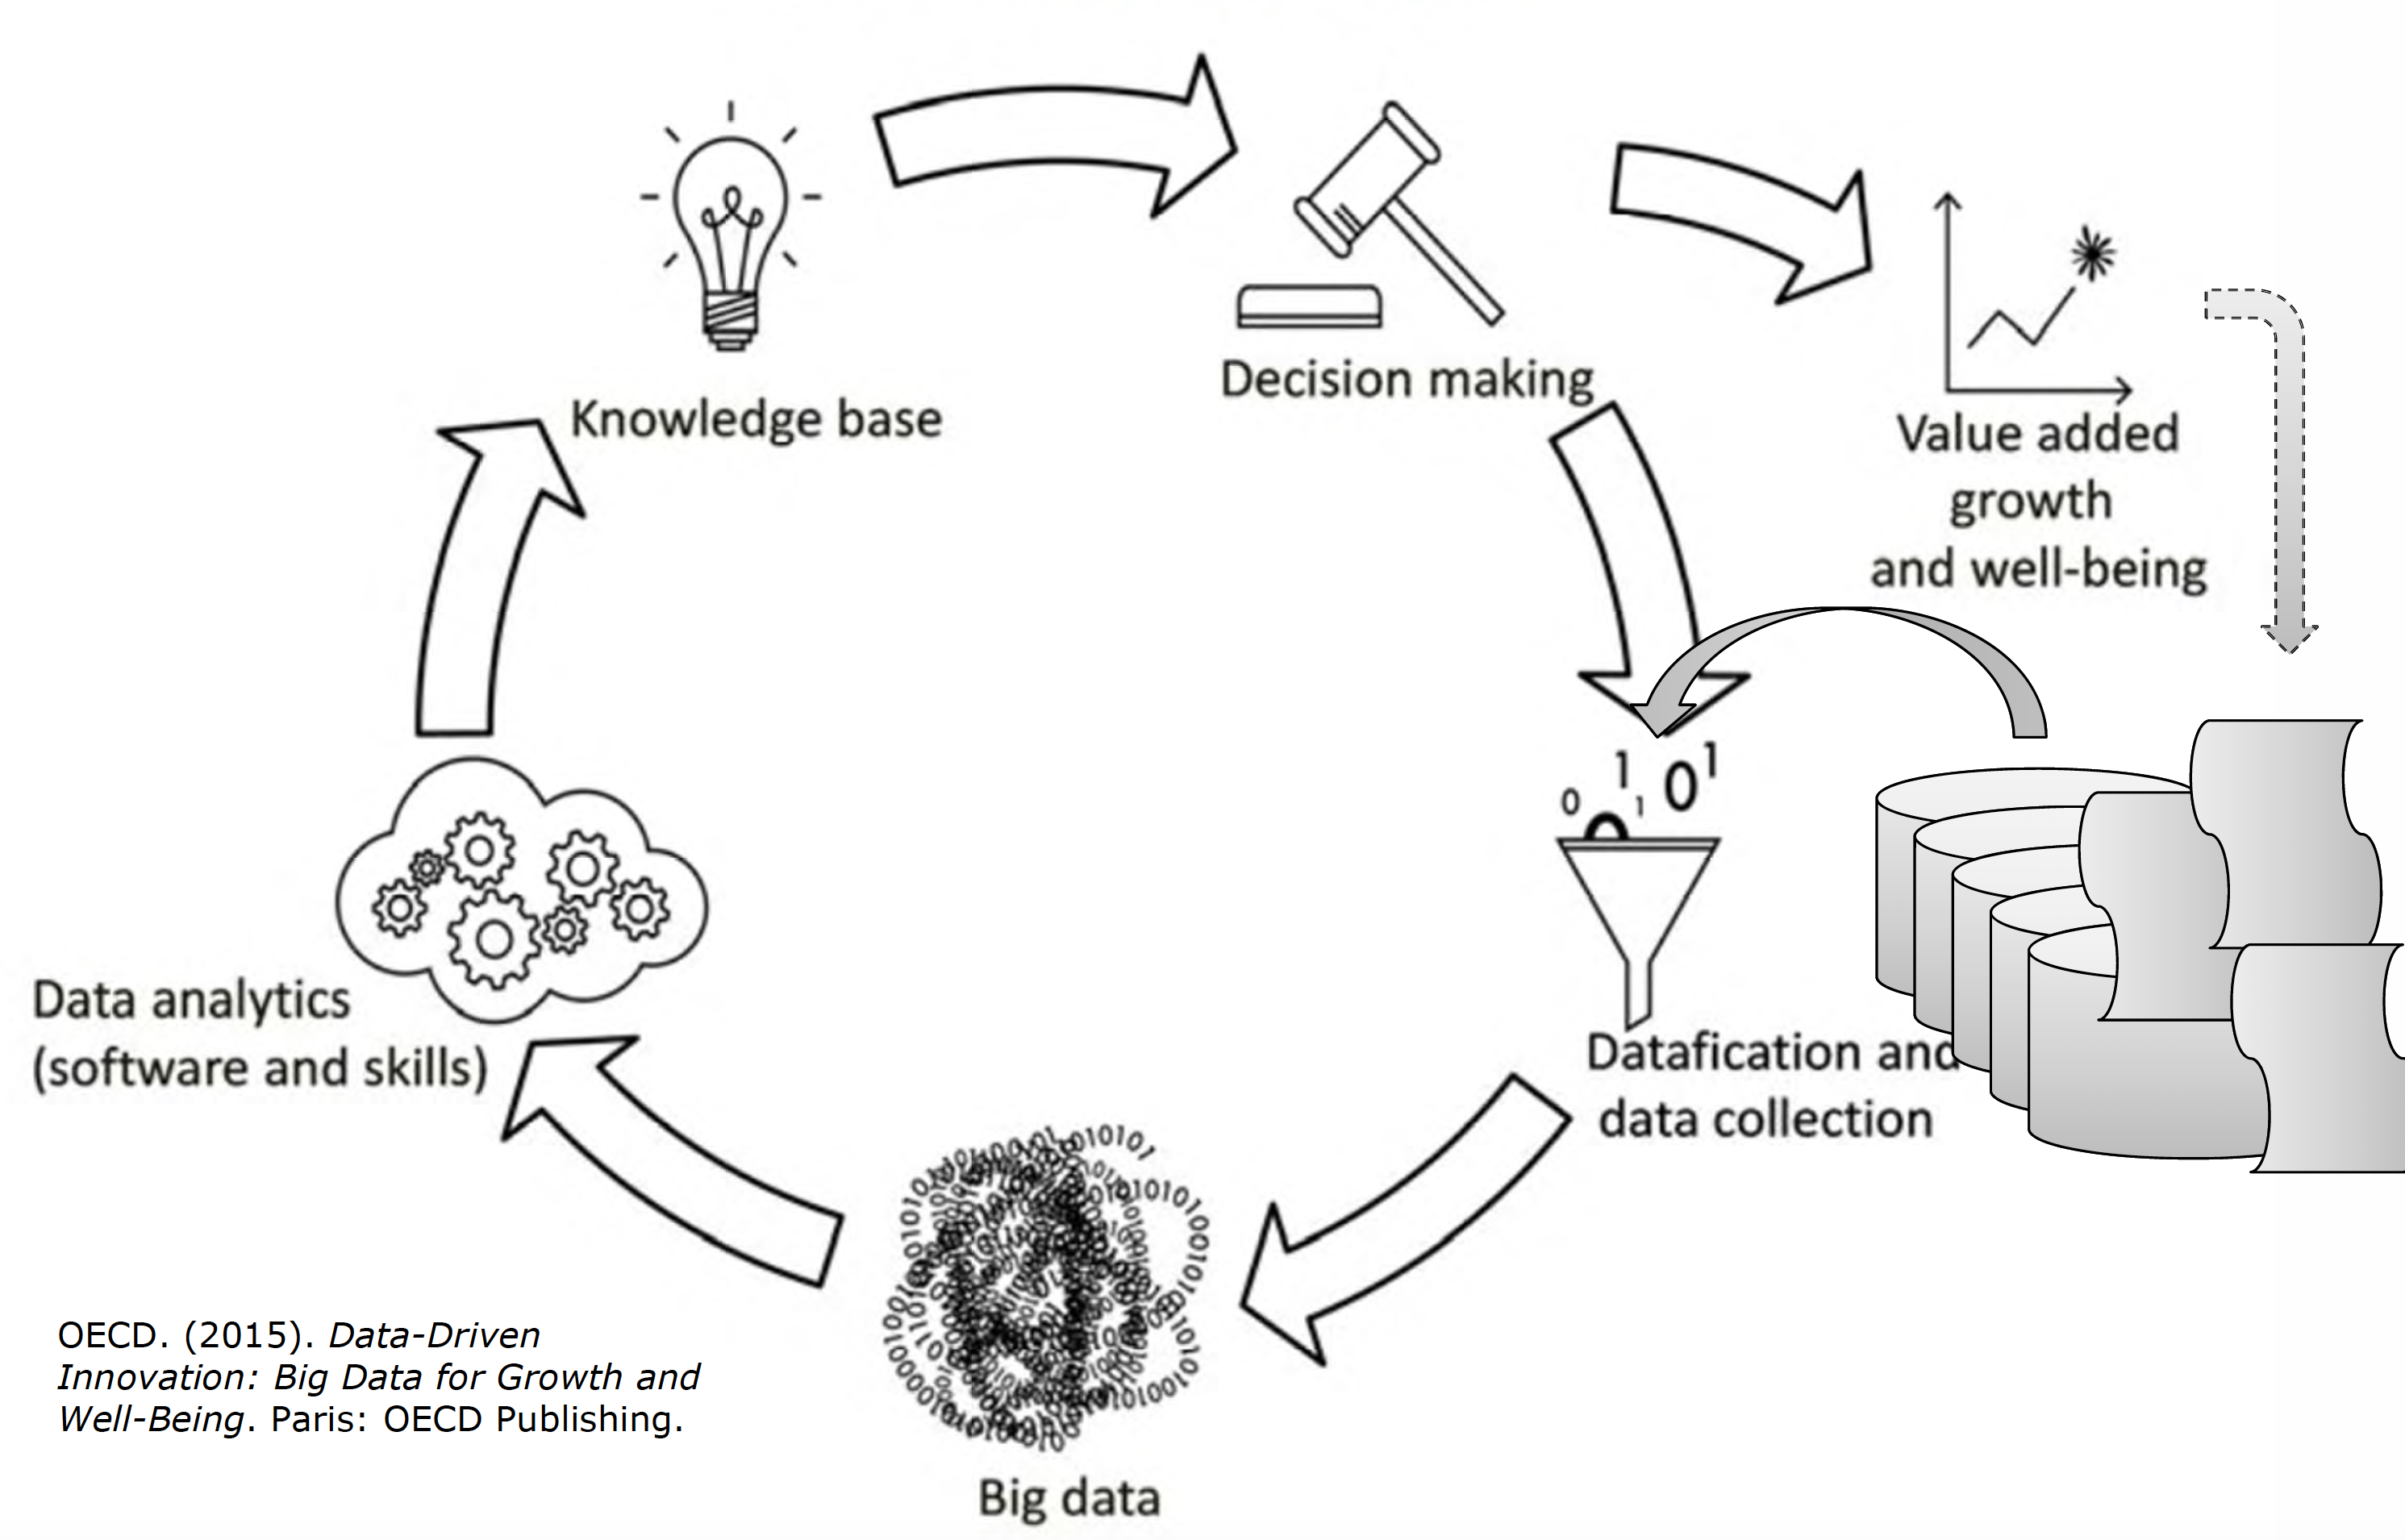
\includegraphics[width=0.5\textwidth]{img/sw01/data_value_cycle.png}
			\caption{Beautiful illustration of the classic data value cycle}
		\end{figure}
	\noindent
		"\textbf{Data Science} is the extraction of actionable knowledge directly from data through a discovery, or hypothesis formulation and hypothesis testing".
		Data Scientists generate knowledge from big data.
		
		\begin{figure}[htb!]
			\centering
			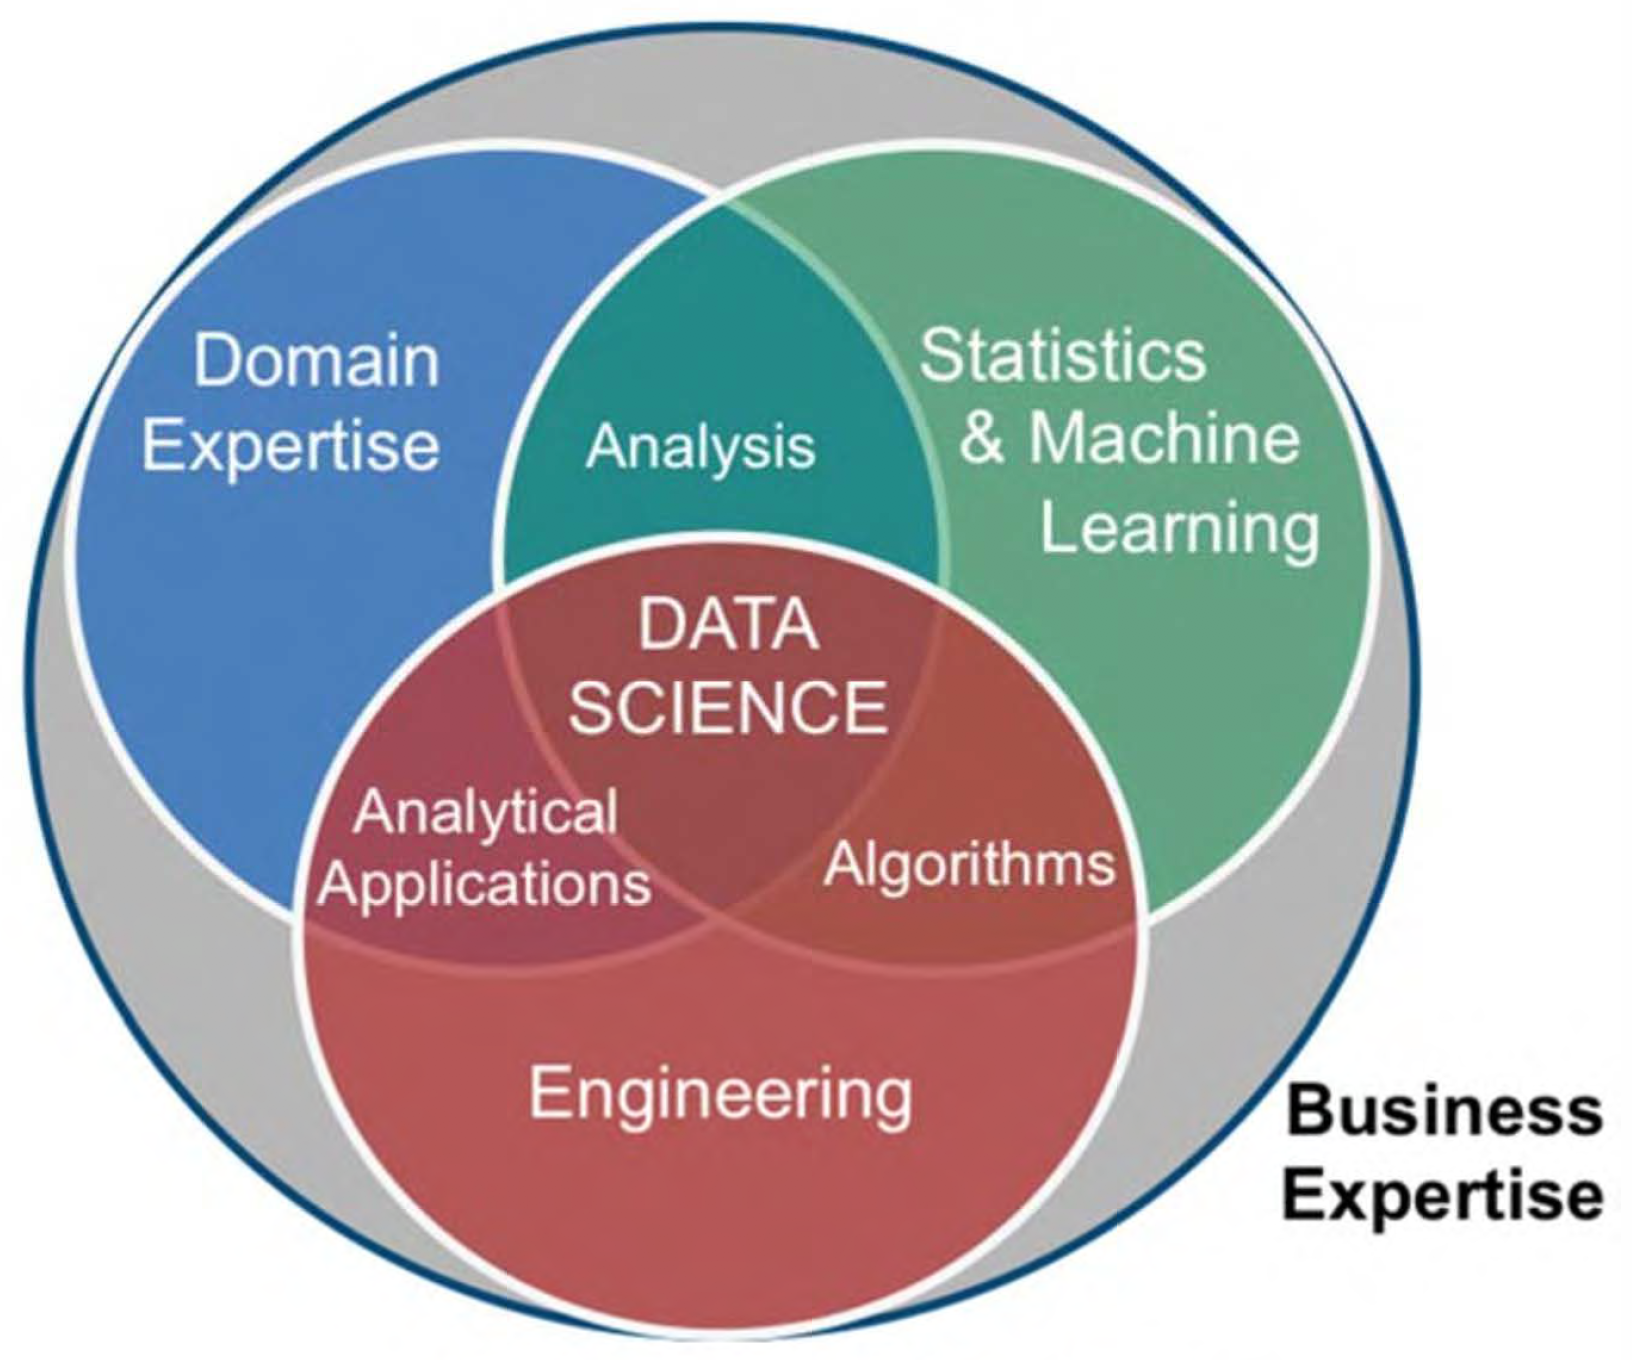
\includegraphics[width=0.3\textwidth]{img/sw01/ds_skills.png}
			\caption{Skills needed in Data Science}
		\end{figure}
	
		\subsection{A Global View on Data Science}
		
		\begin{figure}[htb!]
			\centering
			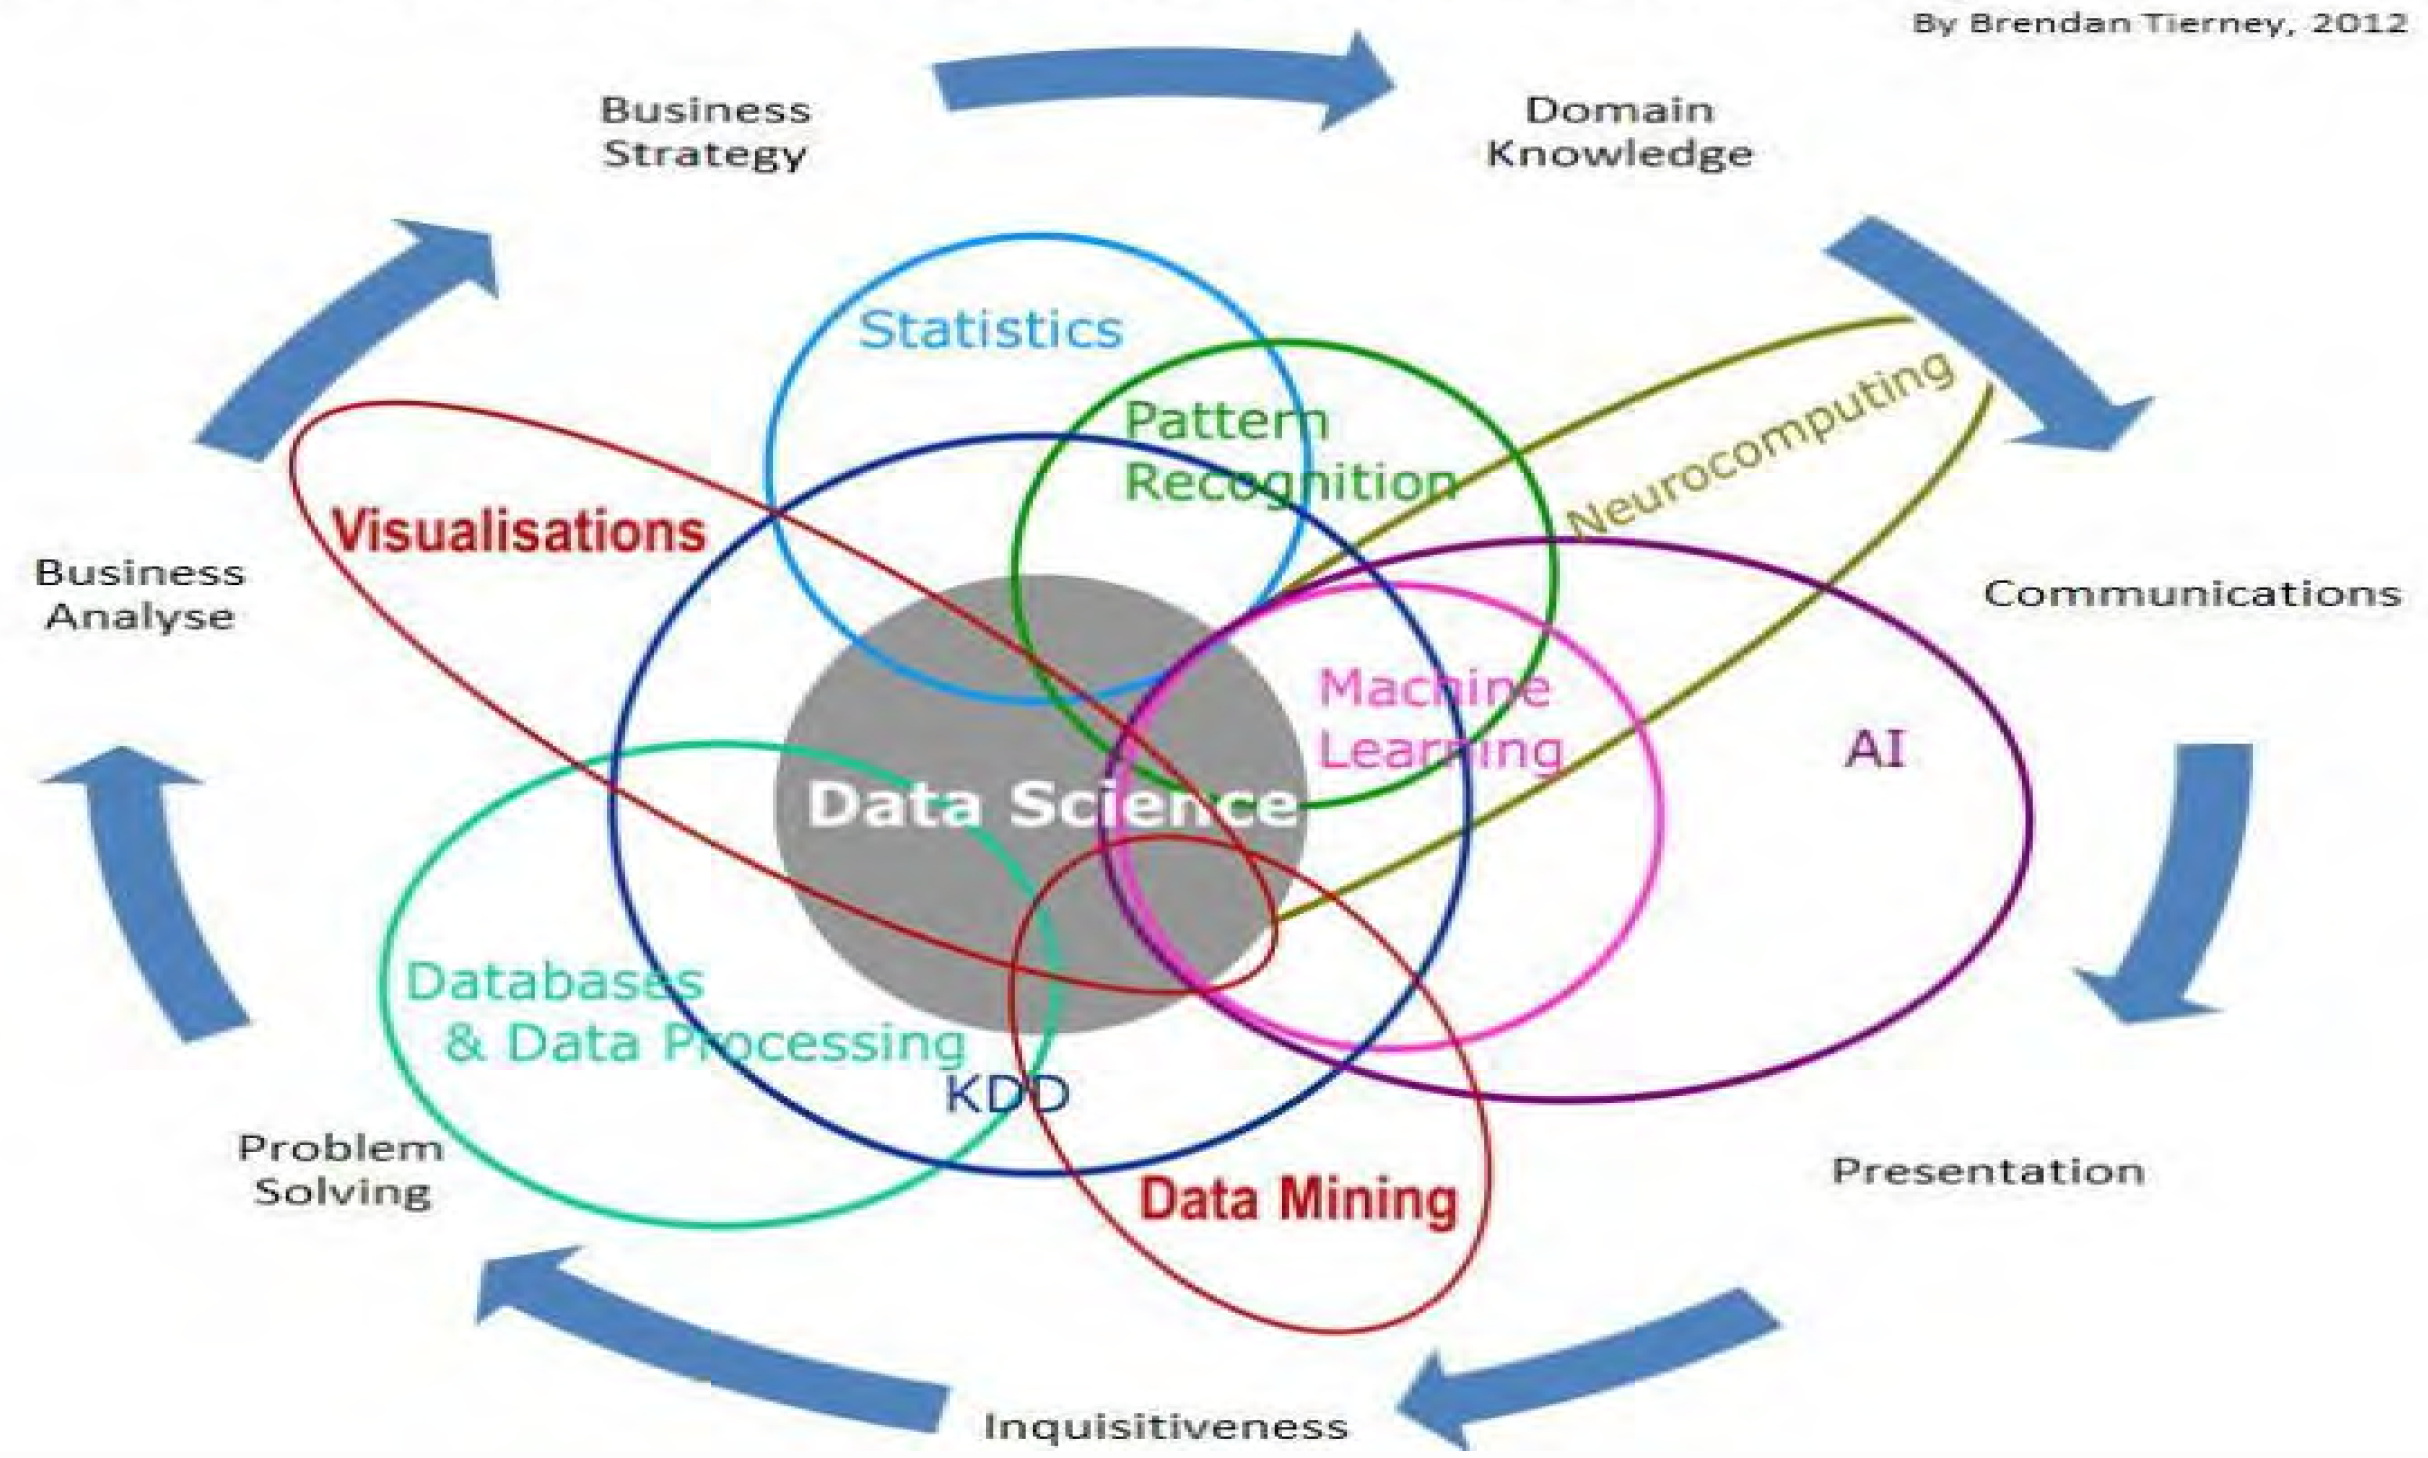
\includegraphics[width=0.5\textwidth]{img/sw01/multidisc.png}
			\caption{Data Science is multidisciplinary}
		\end{figure}
	
		\newpage
		
		\begin{itemize}
			\item \textbf{AI}: programs that perform tasks resembling humans (learn and reason)
			\item \textbf{ML}: algorithms to learn from that data without explicit programming
			\item \textbf{DL}: subset of ML using artificial neural networks for treating vast amount of data (big data)
			\item \textbf{Data Science}: spans the collection, management, analysis and interpretation of large amounts of data with a wide range of applications $\rightarrow$
				make informed decisions based on what was learned
			\item \textbf{EDA} (exploratory data analysis): extract insight from data (outside AI, human based)
		\end{itemize}
	
		\begin{figure}[htb!]
			\centering
			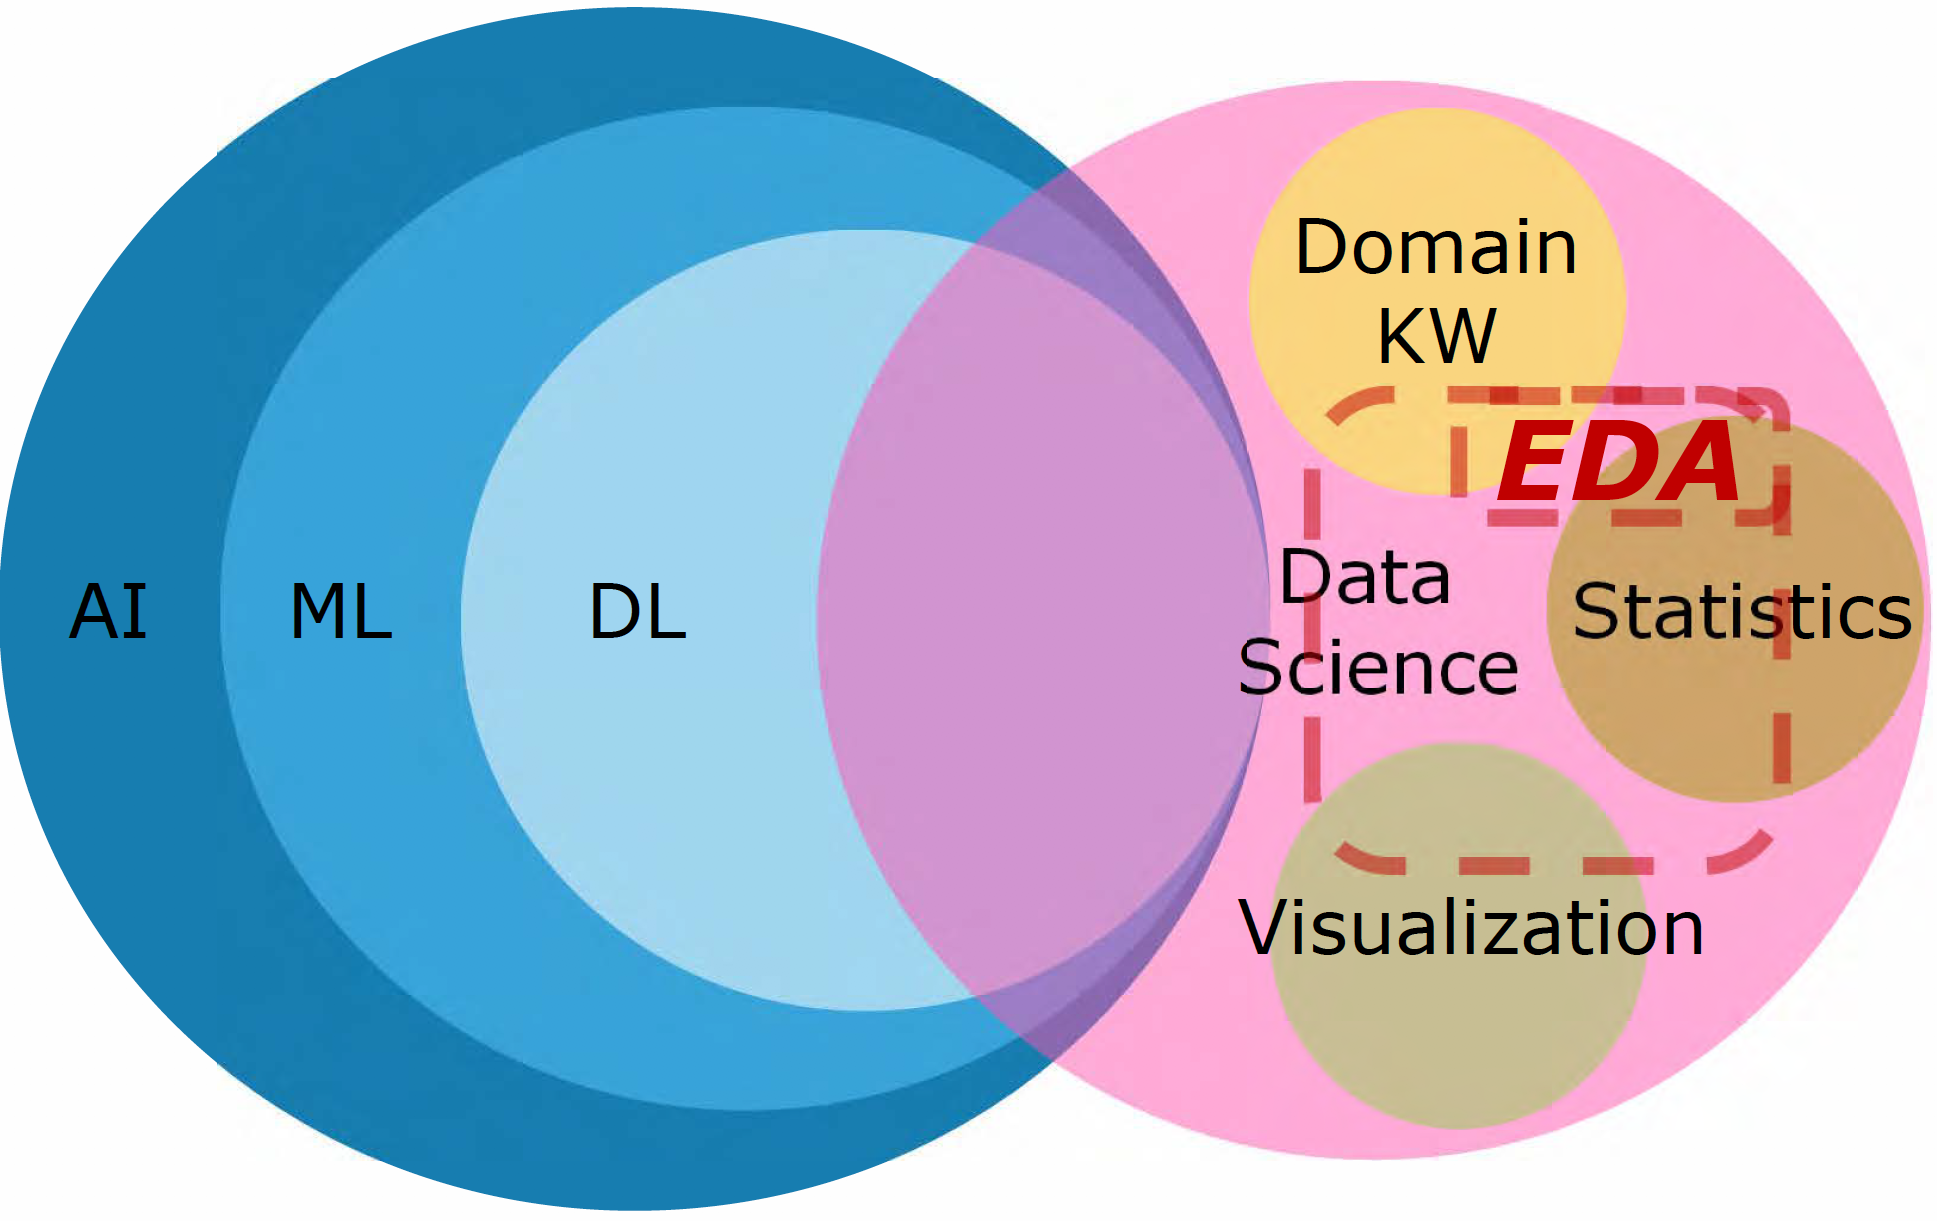
\includegraphics[width=0.4\textwidth]{img/sw01/global_view.png}
			\caption{AI / ML / DL and Data Science}
		\end{figure}
	
		\subsection{Different Concepts in Data Analytics}
		
			\subsubsection{1993 - Online Analytical Processing (OLAP)}
			
			\begin{minipage}[c]{0.3\textwidth}
				\centering
				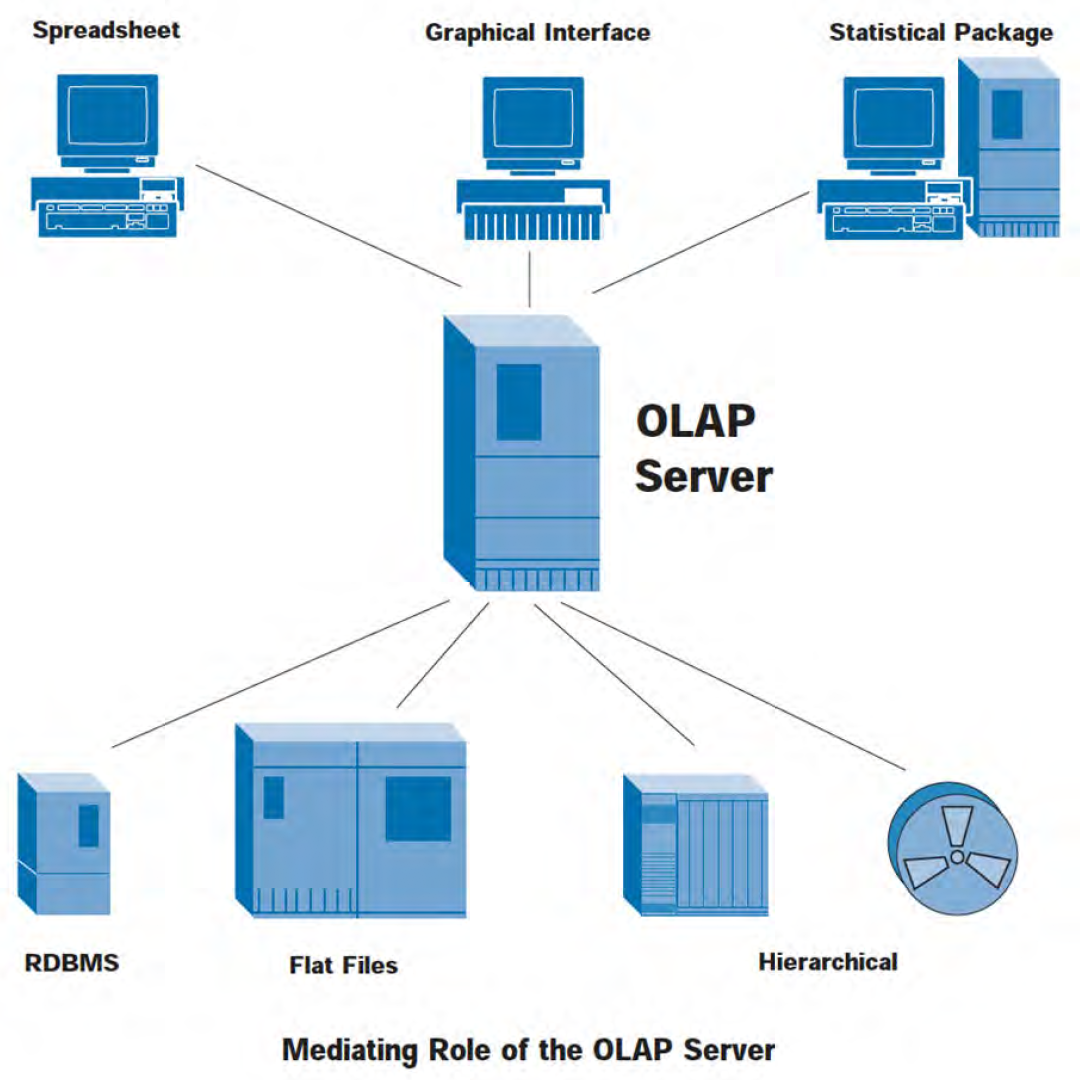
\includegraphics[width=\textwidth]{img/sw01/olap.png}
			\end{minipage}
			\hfill
			\begin{minipage}[c]{0.6\textwidth}
				\begin{itemize}
					\item It's online, not batch (interactive, not programmed in COBOL)
					\item The OLAP system should access the data required to perform the indicated analysis
					\item OLAP tools empower useranalysts to earily perform multi-dimensional analysis, which previously have been avoided because of their perceived complexity.
				\end{itemize}
			\end{minipage}
		
			\subsubsection{1998 - Fuzzy Data Analysis}
			
			\begin{minipage}[c]{0.3\textwidth}
				\centering
				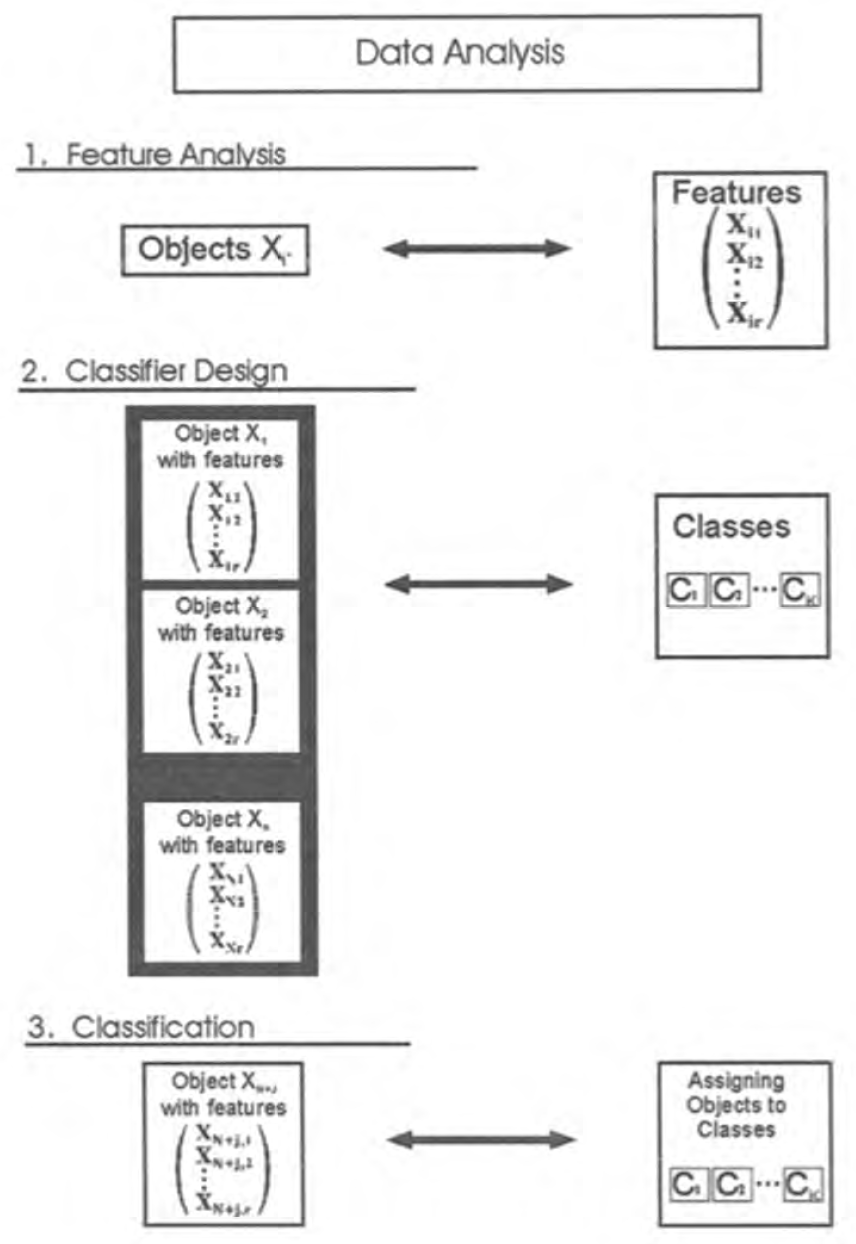
\includegraphics[width=.8\textwidth]{img/sw01/fda.png}
			\end{minipage}
			\hfill
			\begin{minipage}[c]{0.6\textwidth}
				\begin{itemize}
					\item Data analysis can be defined as  \\
						\textbf{search for structure} in data
					\item In data analysis, objects are considered which are described by some attributes
					\item Most of the traditional methods for data analysis assume that patterns to be detected are two-valued
					\item Whenever this is not the case, the relationship between data and classes becomes gradual \\
						$\rightarrow$ Fuzzy Classification
				\end{itemize}
			\end{minipage}
			
			\newpage
			
			\subsubsection{2005 - Data Mining}
			
			\begin{minipage}[c]{0.3\textwidth}
				\centering
				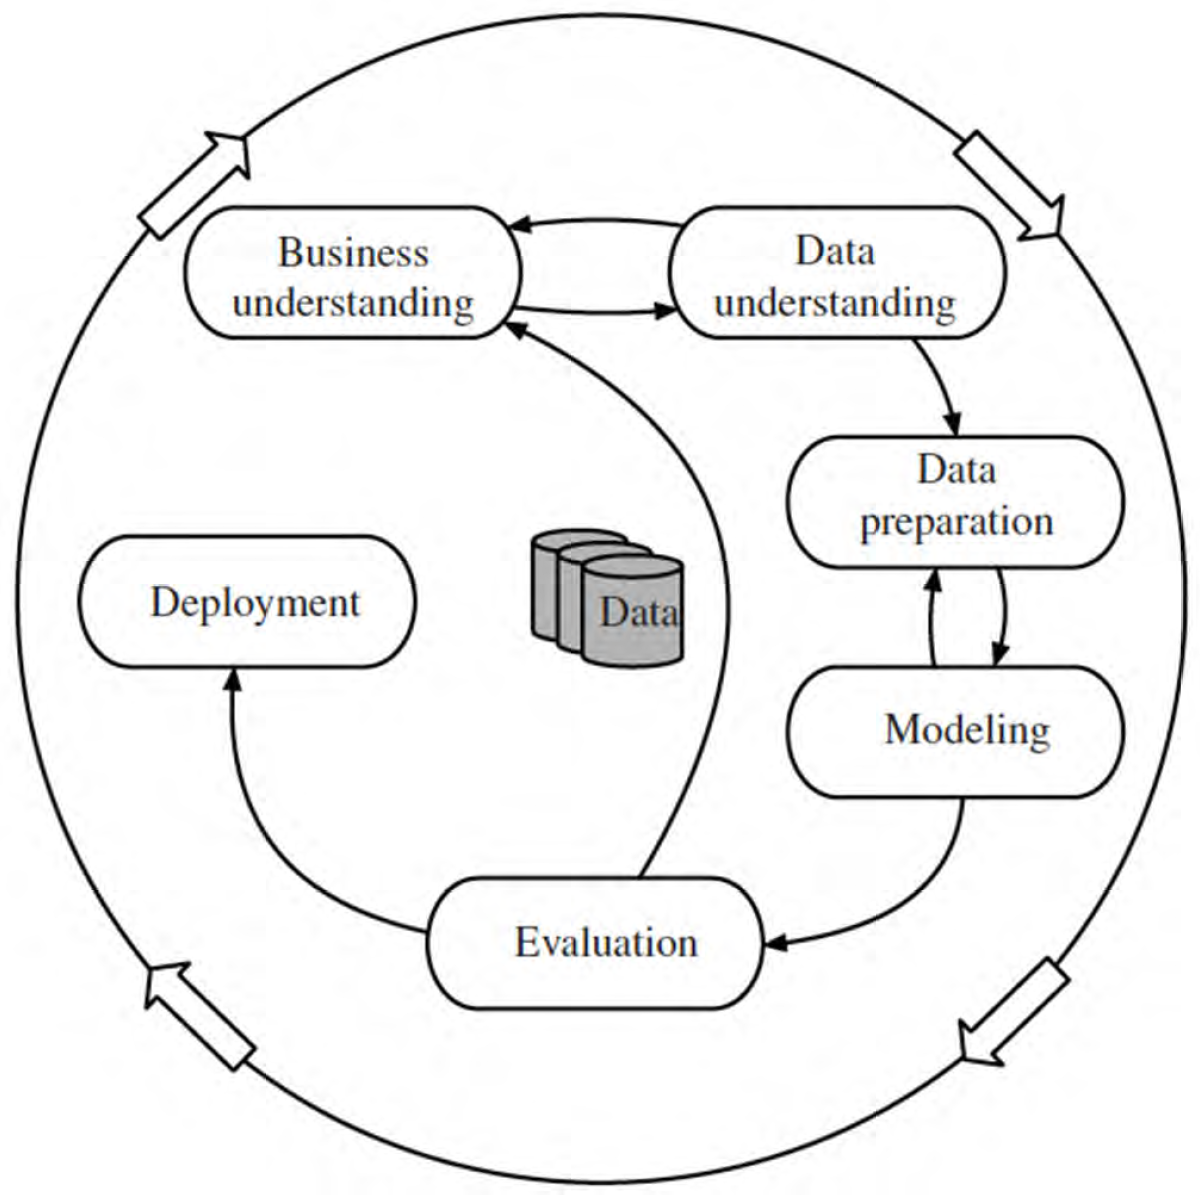
\includegraphics[width=\textwidth]{img/sw01/data-mining.png}
			\end{minipage}
			\hfill
			\begin{minipage}[c]{0.6\textwidth}
				\begin{itemize}
					\item Very similar concept to data science
					\item Machine Learning (modeling) is the technical core of practical data mining applications
					\item Data \textit{Mining} is a business process related to \textit{value} (finding the metaphorical gold nugget)
					\item The lifecycle of a data mining project is defined by the CRISP-DM reference model
				\end{itemize}
			\end{minipage}
		
			\subsubsection{2013 - Predictive Modeling}
			
			\begin{minipage}[c]{0.45\textwidth}
				\centering
				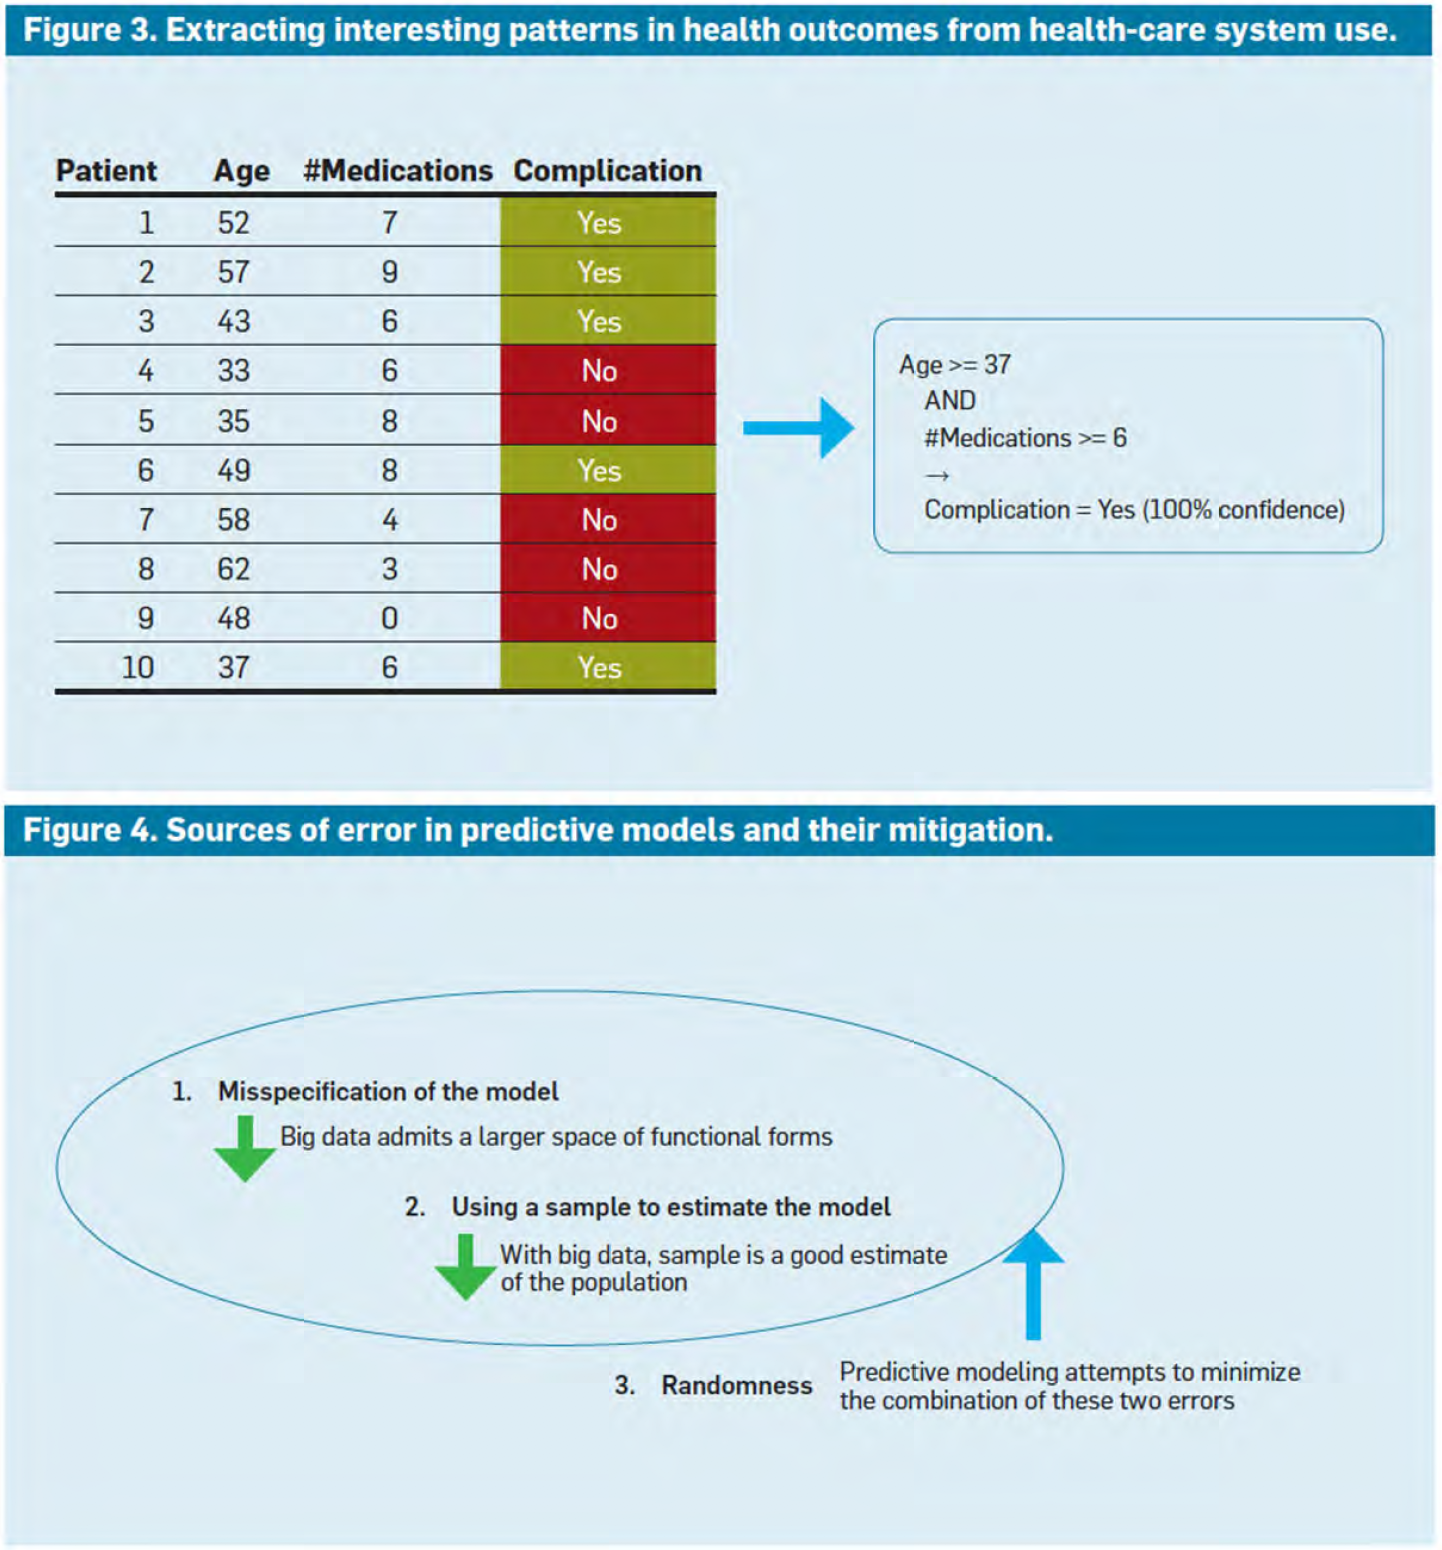
\includegraphics[width=\textwidth]{img/sw01/pred_mod.png}
			\end{minipage}
			\hfill
			\begin{minipage}[c]{0.45\textwidth}
				\begin{itemize}
					\item A common epistemic requirement in assessing whether new knowledge is actionable for decision making in its \textit{predictive power}, not just its ability to explain the past.
					\item The requirement on predictive accuracy on observations that will occur in the future is a key consideration in data science.
				\end{itemize}
			\end{minipage}
		
			\subsubsection{2013 - Data Driven Decision Making}
			
			\begin{minipage}[c]{0.3\textwidth}
				\centering
				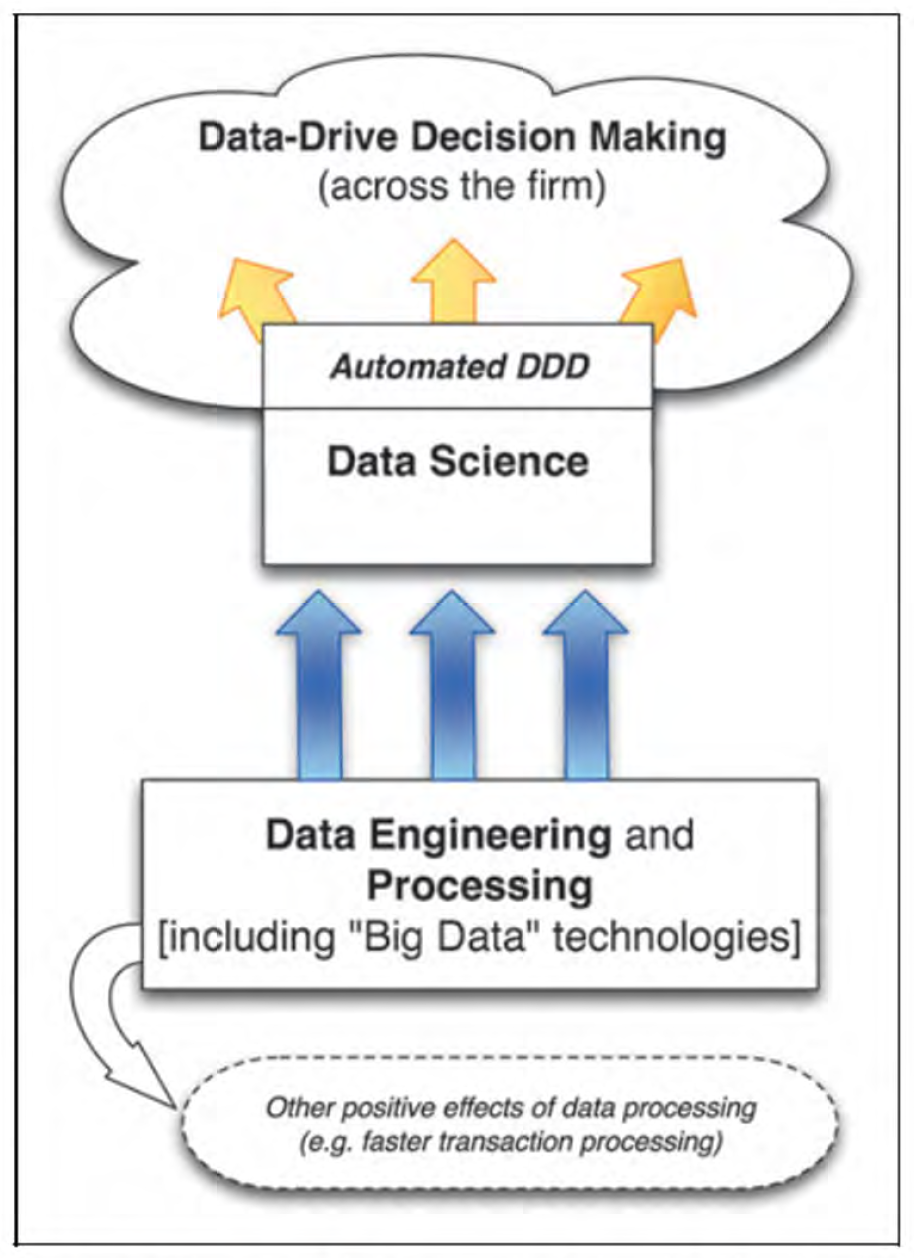
\includegraphics[width=\textwidth]{img/sw01/data_driven.png}
			\end{minipage}
			\hfill
			\begin{minipage}[c]{0.6\textwidth}
				\begin{itemize}
					\item Data science involves much more than just data-mining algorithms.
					\item Successful data scientists must be able to view business problems form a \textit{data perspective}.
				\end{itemize}
			\end{minipage}
		
			\newpage
		
	\section{Intro to R and Exploratory Data Analysis (EDA)}
	
		\subsection{Intro to R}
		
		\begin{itemize}
			\item \textbf{R} ist a software and programming language for statistical applications and graphics
			\item It's an implementation of the programming language S, with some extensions
			\item It provides functions for linear/non-linear modelling, classical statistical tests, time-series analysis, classification, clustering etc.
			\item \textbf{RStudio} is an integrated development environment (IDE) for R
		\end{itemize}
	
			\subsubsection{Basic Operation in R}
			
			\begin{itemize}
				\item Assignment:\\
					\texttt{my\_var <- 46, nr <- 38} \\
					(You can also use \texttt{copy my\_var = 46}, but it is not suggested)
				\item Printing (explicit and implicit): every line with only a name of an object \\
					Implicit: \texttt{my\_var} \\
					Explicit using functions like print: \texttt{print(my\_var)}
				\item Arithmetic operators: \\
					\texttt{4 + 5} \\
					\texttt{2 \^{} 3 - 7 \%\% 3 - 2 \^{} (3 - 7 \%\% 3)} etc. etc. etc.
				\item Control flow, conditionals, loops can be used as in any other language \\
					\texttt{for (i in 1:10) {print(i)}} \\
					\texttt{while (nr < 42) {print("We have "+str(nr)+" : still space..."); nr=nr+1}}
			\end{itemize}
	
		\subsection{What is EDA}
		
		\begin{itemize}
			\item Exploratory Data Analysis is the
				\begin{itemize}
					\item critical process of performing initial investigations on data so as to
						\begin{itemize}
							\item discover patterns
							\item spot anomalies
							\item test hypothesis
							\item check assumptions
						\end{itemize}
					\item with the help of \textbf{summary statistics} and \textbf{graphical representations}
				\end{itemize}
		\end{itemize}
	\noindent
		The use of a statistical model is not mandatory, in this step, even if it is normally adopted to test hypotheses and check assumptions.
		For anomalies and patterns discovery, correlations (represented into the correlation matrix) and distribution (represented with box and whisker diagrams) are the usual approaches.
		
		\begin{figure}[htb!]
			\centering
			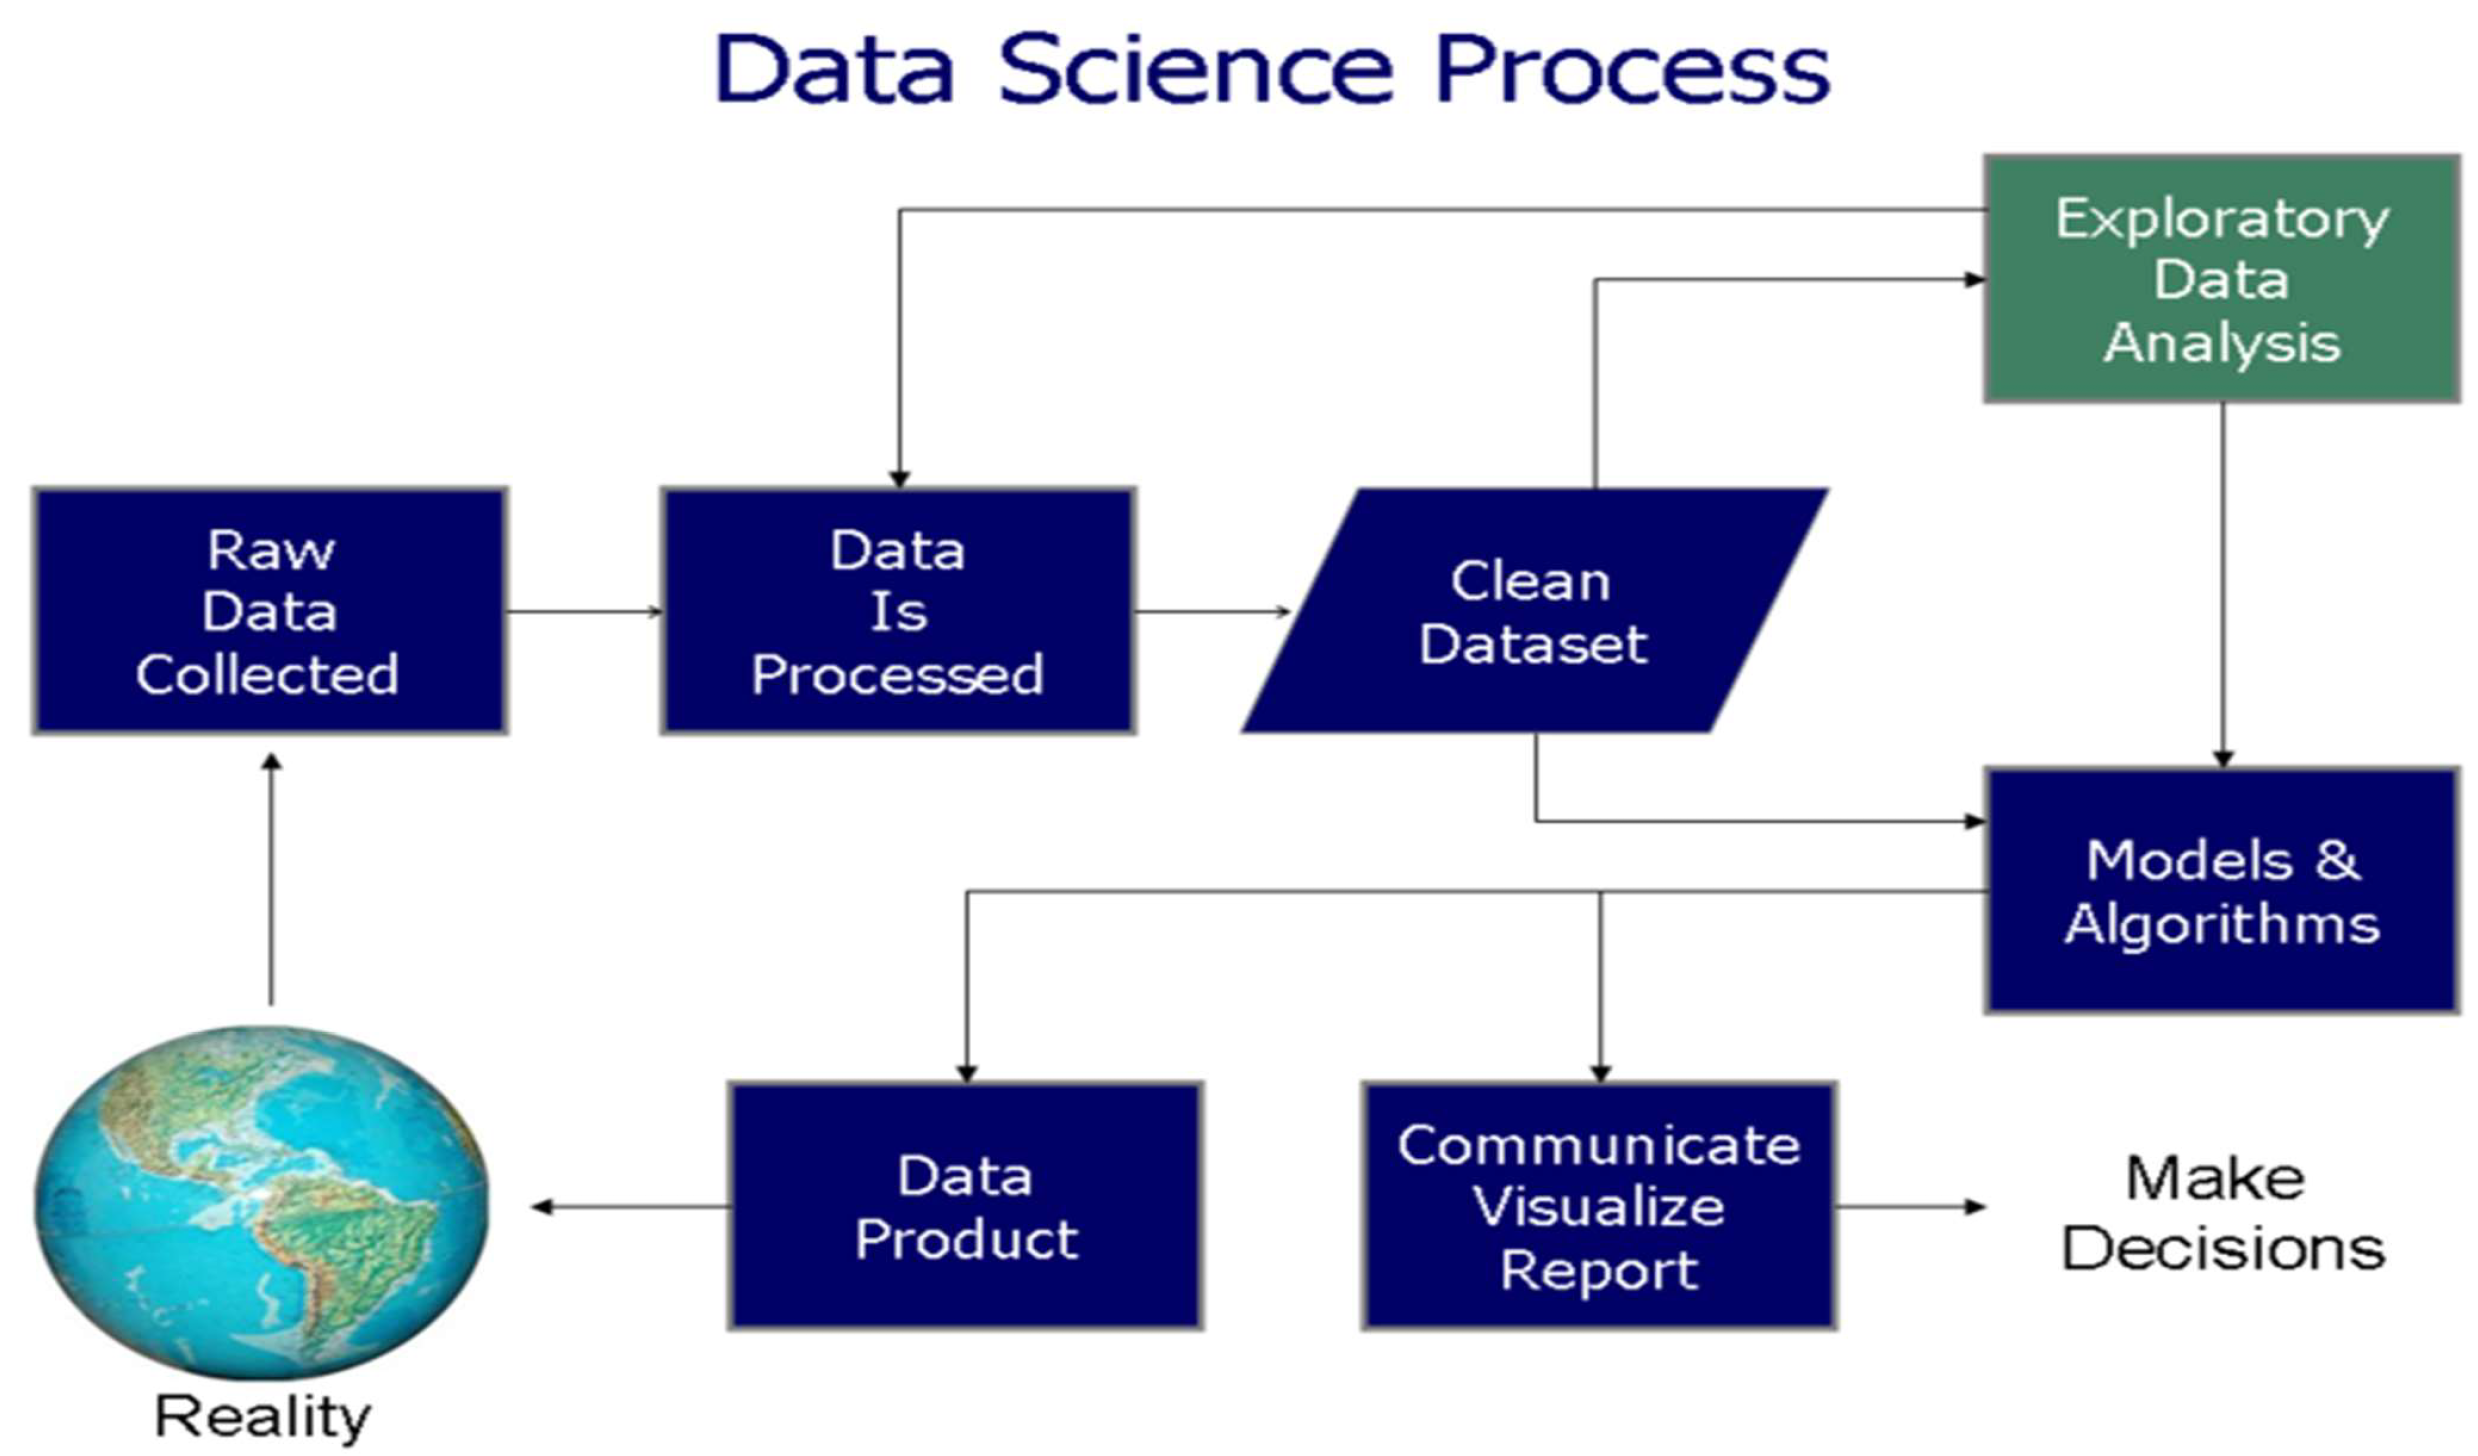
\includegraphics[width=.7\textwidth]{img/sw02/eda_context.png}
			\caption{EDA in the context of Data Science}
		\end{figure}
	
			\newpage
	
			\subsubsection{EDA process "in practice"}
			
			\begin{itemize}
				\item EDA is an iterative cycle
				\item Process:
					\begin{itemize}
						\item Generate questions about the data
						\item Search for answers by visualizing, transforming and modelling the data
						\item Use the insights to refine the questions and/or generate new questions
					\end{itemize}
				\item Start with many ideas...
				\item some will be evidently useless and other will end up in a dead end
				\item a few of them will help to have a better understanding of the data/process
				\item repeat with generating other ideas until the insight is enough
				\item then you can apply the model to the data for forecasting and process explanation
				\item EDA also allows you to verify/test the quality of your data
			\end{itemize}
		
		\subsection{Data Import / Transform / Link}
		
			\subsubsection{Data Import}
			
			\begin{itemize}
				\item R provides importing functions, depending on the format of the data source:
					\begin{itemize}
						\item CSV / TSV / delimited texts: \texttt{read\_csv()} \& \texttt{read\_csv2()} (semicolon), \texttt{read\_tsv()}, \texttt{read\_delim()}
						\item Fixed width columns: \texttt{read\_fwf()} \& \texttt{read\_table()}
						\item Logs (e.g. webserver logs): \texttt{read\_log()}
					\end{itemize}
			\end{itemize}
			These are all similar in terms of parameters, examples:
			
			\begin{lstlisting}
read_delim(file, delim, quote = "\", escape_backslash = FALSE, escape_double = TRUE,
col_names = TRUE, col_types = NULL, locale = default_locale(), na = c("", "NA"),
quoted_na = TRUE, comment = "", trim_ws = FALSE, skip = 0, n_max = Inf, guess_max =
			\end{lstlisting}
			
			\subsubsection{Data Transform (example dataset)}
		
			Example dataset loaded from: \href{https://archive.ics.uci.edu/ml/machine-learning-databases/auto-mpg/}{\textit{\underline{Auto MPG Data Set}}}

			\begin{lstlisting}
> library(tidyverse)
> DS <- read.table("C:/Users/JumpStart/Downloads/auto-mpg.data",
quote="\", comment.char="")
> names(DS) <-
c("mpg","cylinders","displacement","horsepower","weight","acceleration","
model year","origin","car name")
> DS <- as_tibble(DS); attach(DS); View(DS)
			\end{lstlisting}
			
			\newpage
			
			\subsubsection{Data Transform}
		
			\begin{itemize}
				\item Filter rows with \texttt{filter()}
					\begin{itemize}
						\item subset observations based on their values \\
						\texttt{filter(DS, weight > 3500)} or \texttt{filter(DS, DS\$weight > 3500)}
					\end{itemize}
				\item Arrange rows with \texttt{arrange()}
					\begin{itemize}
						\item changes the order of rows \\
						\texttt{arrange(DS, desc(DS\$acceleration))}
					\end{itemize}
				\item Select columns with \texttt{select()}
					\begin{itemize}
						\item Subset columns with position and/or negative condition (by name or index) \\
						\texttt{select(DS, -1)} \\
						\texttt{select(DS, 2, 3, 4)} \\
						\texttt{select(DS, c(mpg, 5))}
					\end{itemize}
				\item Add new variables with \texttt{mutate()} 
					\begin{itemize}
						\item Allow to create new dimension(s) \\
						\texttt{mutate(DS, a4w = acceleration/weight, pre75 = as.numeric(DS\$'model year' < 75))}
					\end{itemize}
				\item Grouped summaries with \texttt{summarise()}
					\begin{itemize}
						\item Allows to compute aggregate metrics \\
						\texttt{summarise(group\_by(DS, 'model year'), mean\_display = mean(displacement), sd\_displ = sd(displacement), n=n()}
					\end{itemize}
			\end{itemize}
			\vspace{1em}
			\begin{itemize}
				\item All verbs work similarly:
					\begin{itemize}
						\item The first argument is a dataframe
						\item The subsequent arguments describe what to do with the data frame, using the variable names (without quotes)
						\item The result is a new data frame
					\end{itemize}
			\end{itemize}
		
			\subsubsection{Data "Linkage"}
			
			Some prices of cars of the 70's: \href{http://www.thepeoplehistory.com/70scars.html}{\textit{\underline{70's Cars}}}. \\
			This data is imported into a new tibble and we will try to use it for creating another View for exploring the relationship between cost, year, power and mpg.
			
			\begin{lstlisting}
> car_cost <-read_delim("C:/Users/JumpStart/switchdrive/__/DASB/SW02/car_197x_costs_2.csv", 
		delim = "-", 
		escape_double = FALSE, 
		na = "NA", 
		trim_ws = TRUE, 
		col_types = cols(`Car Name` = col_factor(), 
		Price = col_character(), 
		Location = col_character(), 
		`Matriculation Year` = col_integer()))
> car_cost <- as_tibble(car_cost)
> car_cost <- mutate(car_cost, Location = sapply(Location,as.factor))
> car_cost <- mutate(car_cost, Price = as.integer(str_replace(str_sub(Price, 2, -1),",","")))
> View(car_cost)
			\end{lstlisting}
	
			\begin{figure}[htb!]
				\centering
				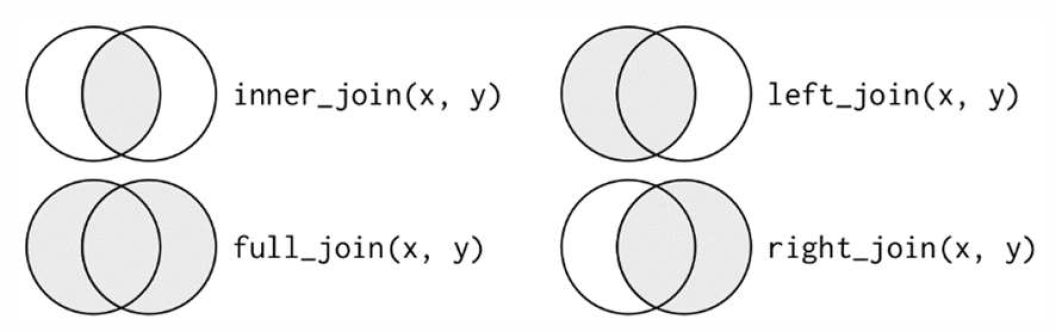
\includegraphics[width=.7\textwidth]{img/sw02/data_linkage.png}
				\caption{R functions to link data frames with each other}
			\end{figure}
	
			\newpage
		\noindent
			There are different types of R functions for linking tibbles/dataframes (\textasciitilde datasets)
					\begin{itemize}
						\item \textbf{Mutating} joins allows to combine variable from two tables
							\begin{itemize}
								\item \texttt{inner\_join(x, y, by = keys)} \\
								matches pairs of observations whenever their keys are equal
								\item Outer join keeps observations that appear in at least one of the tables.
									There are three types of outer joins:
										\begin{itemize}
											\item \texttt{left\_join(x, y, by = keys)} \\
												keeps all observations in x
											\item \texttt{right\_join(x, y, by = keys)} \\
												keeps all observations in y
											\item \texttt{full\_join(x, y, by = keys)} \\
												keeps all observations in x and y
										\end{itemize}
							\end{itemize}
						\item \textbf{Filtering} joins allow to restrict the set of row from the 1$^{st}$ table
							\begin{itemize}
								\item \texttt{semi\_join(x, y, by = keys)} \\
									keeps all observations in x that have a match in y
								\item \texttt{anti\_join(x, y, by = keys)} \\
									drops all observations in x that have a match in y
							\end{itemize}
						\item \textbf{Set Operations} (work on complete rows, comparing each variable values.
							Inputs needs the same variables, for treating observations like sets)
							\begin{itemize}
								\item \texttt{intersect(x, y)} \\
									return only observations in both x and y
								\item \texttt{union(x, y)} \\
									return unique observations in x and y
								\item \texttt{setdiff(x, y)} \\
									return observations in x, but not in y
							\end{itemize}
					\end{itemize}
				
			\subsubsection{Applying data loading/transforming/linking}
			
			\begin{itemize}
				\item Find one or more data sources you are interested into (\href{https://archive.ics.uci.edu/ml/datasets.php}{UCI ML Repository} / \href{https://www.kaggle.com/datasets}{Kaggle})
				\item Start the EDA "mindset":
					\begin{enumerate}
						\item What I believe about the data / what I would like to discover \\
							$\rightarrow$ Make hypotheses and formulate assumptions
						\item Think how this can be supported by data $\rightarrow$ experiment
						\item Run the experiment to verify
						\item Acquire new knowledge that can help you improve step 1
					\end{enumerate}
				\item Repeat the process at least 3 times \\
				\textit{(Optional: short report of the process you followed, document it in a short presentation)}
			\end{itemize}
		
	\section{ggplot2 and its usage in EDA}
	
		\subsection{ggplot2 - Intro}
		
		\begin{itemize}
			\item Used with the library "ggplot2" \\
				\texttt{library(ggplot2)}
			\item Simple usage example: \\
				\texttt{plot <- ggplot(data = mpg, mapping = aes(x = mpg\$hwy))} \\
				plot + geom\_histogram()
			\item ggplot 2 package:
				\begin{itemize}
					\item produces layered statistical graphics.
					\item uses an underlying "grammar" to build graphs layer-by-layer rather than providing premade graphs
					\item is easy enough to use without any exposure to the underlying grammar, but is even easier to use once you know the grammar
					\item allows the user to build a graph from concepts rather than recall of commands and options
				\end{itemize}
		\end{itemize}
	
		\newpage
	
		\subsection{ggplot2 - layer after layer}
		
		\begin{itemize}
			\item The initial call to ggplot does create the graph, but no content: \\
				\texttt{ggplot(data = mpg)} \\
				\texttt{ggplot(data = mpg, mapping = aes(x = mpg\$hwy))} \\
				\texttt{ggplot(data = mpg, mapping = aes(x = mpg\$hwy, y = mpg\$dipl))}
			\item We need to add a layer by using + (or collect the partial graph in an object) \\
				\texttt{p <- ggplot(data = mpg)} \\
				\texttt{p + geom\_histogram(mapping = aes(x = mpg\$hwy))}
			\item Parameters set into the ggplot() call are inherited by every other layer, but can be overridden, if needed \\
				\texttt{p <- ggplot(data = mpg)} \\
				\texttt{p <- p + geom\_histogram(mapping = aees(x = mpg\$hwy))} \\
				\texttt{p} \\
				\texttt{p +  geom\_violin(mapping = aes(y = mpg\$displ))}
		\end{itemize}
	
		\subsection{Elements of grammar of graphics}
		
		\begin{itemize}
			\item \textbf{Data}: variables mapped to aesthetic features of the graph.
			\item \textbf{Geoms}: objects / shapes on the graph.
			\item \textbf{Stats}: statistical transformations that summarize data (e.g. mean, confidence intervals).
			\item \textbf{Scales}: mappings of aesthetic values to data values. 
				Legends and axes visualize scales.
			\item \textbf{Coordinate systems}: the plane on which data is mapped on the graphic.
			\item \textbf{Faceting}: splitting the data into subsets to create multiple variations of the same graph (paneling). 
		\end{itemize}
	
		\subsection{Aesthetics}
		
		\begin{itemize}
			\item Visual properties of objects on the graph (depends on the geom*)
			\item Commonly used aesthetics:
				\begin{description}
					\item[x] positioning along x-axis
					\item[y] positioning along y-axis
					\item[color] color of objects; for 2D-objects: the color of the object's outline (compare to fill below)
					\item[fill] fill color of objects
					\item[linetype] how lines should be drawn (solid, dashed, dotted etc.)
					\item[shape] shape of markers in scatter plots
					\item[size] how large objects appear
					\item[alpha] transparency of objects (value from 0 [transparent] to 1 [opaque])
				\end{description}
		\end{itemize}
	
		\subsection{Geoms}
		
		\begin{itemize}
			\item Geometric shapes produced for the plot.
				\begin{itemize}
					\item \texttt{geom\_bar()}: bars with bases on the x-axis
					\item \texttt{geom\_boxplot()}: boxes and whiskers
					\item \texttt{geom\_density()}: density plots
					\item \texttt{geom\_histogram()}: histogram
					\item \texttt{geom\_line()}: lines
					\item \texttt{geom\_point()}: points (scatterplot)
					\item \texttt{geom\_rug()}: rug plot (2D display with the two 1D marginal distributions)
					\item \texttt{geom\_smooth()}: smoothed conditional means
					\item \texttt{geom\_text()}: text
				\end{itemize}
		\end{itemize}
	
		\newpage
		
		\subsection{Stats \& Scales}
		
		\begin{itemize}
			\item \textbf{Stats} $\rightarrow$ statistically transform data, usually as some form of summary (e.g.: mean, standard deviation, confidence interval etc.).
				Each stat function is associated with a default geom, so no geom is required for shapes to be rendered.
			\item \textbf{Scales} $\rightarrow$ control how a plot maps data values to the visual values of an aesthetic
				\begin{itemize}
					\item \texttt{scale\_color\_manual()}: \\
						define an arbitrary color scale, by scecifying each color manually
					\item \texttt{scale\_color\_hue()}: \\
						define an evenly-spaced color scale, by specifying a range of hues and the number of colors on a scale
					\item \texttt{scale\_shape\_manual()} \\
						define an arbitrary shape scale, by specifying each shape manually
				\end{itemize}
			\item Scales can also be applied to axes:
				\begin{itemize}
					\item \texttt{scale\_x\_continuous()} \\
						map continuous to visual values - \texttt{scale\_x\_discrete()}
					\item \texttt{scale\_x\_date(labels = date\_format("\%m/\%d"), breaks = date\_breaks("2 weeks"))}: \\
						treat x values as dates - scale\_x\_datetime()
					\item \texttt{scale\_x\_log10()}: \\
						plot x on log10 scale
					\item \texttt{scale\_x\_reverse()}: \\
						reverse direction of x-axis
					\item \texttt{scale\_x\_sqrt()}: \\
						plot x on square root scale
				\end{itemize}
		\end{itemize}
	
		\subsection{ggplot2 - Initial Example}
		
		\begin{lstlisting}
ggplot(diamonds, aes(x=carat, y=price, color=cut)) +
	geom_point() +
	scale_color_manual(
	values=c("red", "yellow", "green", "blue", "violet")
) +
scale_y_continuous(
	breaks=c(0,2500,5000,7500,10000,12500,15000,17500),
	labels=c(0,2.5,5,7.5,10,12.5,15,17.5),
	name="price(thousands of dollars)"
)
		\end{lstlisting}
		
		\begin{figure}[htb!]
			\centering
			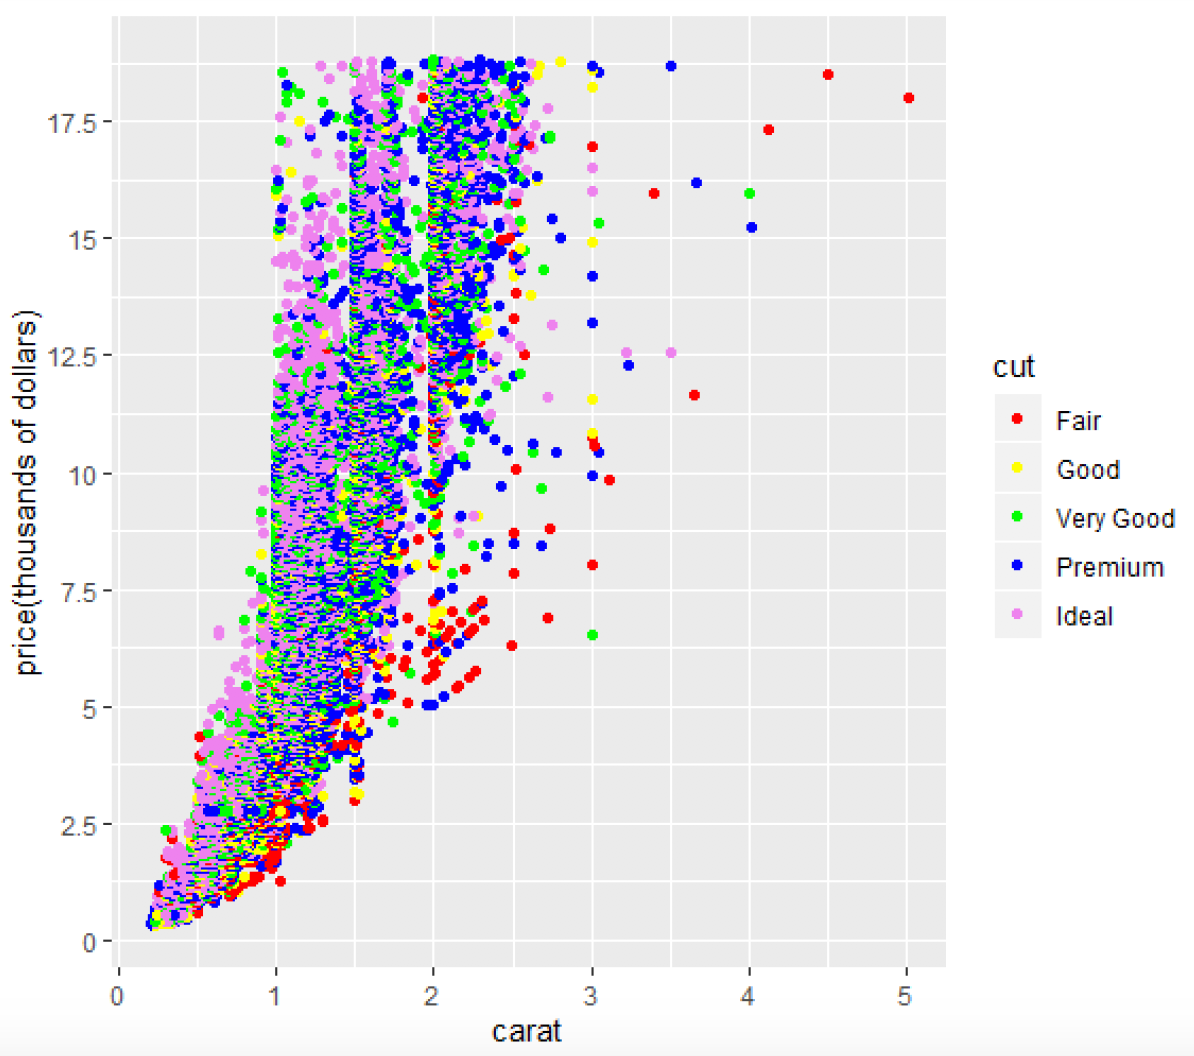
\includegraphics[width=.5\textwidth]{img/sw03/example_01.png}
			\caption{Rendered graph for Initial Example}
		\end{figure}
	
		\newpage
		
		\subsection{Coordinate System \& Faceting}
		
		\begin{itemize}
			\item \textbf{Coordinate system}: set the planes for objects positioning on the plot
			\item Cartesian is the most diffused and used by default.
				Other coordinate systems would be:
				\begin{itemize}
					\item polar
					\item flipped Cartesian
					\item fixed-ratio Cartesian
					\item Map projections (mercatore, lagrange)
				\end{itemize}
			\item \textbf{Faceting}: divide the graph into subgraphs (panels), using variable values
				\begin{itemize}
					\item \texttt{facet\_wrap($\sim$\{vars\})}: \\
						create a multirow panel of plots, \texttt{\{vars\}} represents a list of splitting variables, separated by +
					\item \texttt{facet\_grid(\{vars\}$\sim$\{vars\})}: \\
					row-splitting variable before, the column-splitting variable after
				\end{itemize}
			\item Other aspects include the teming, position adjustment, labels and legends, zooming and the graph savings (ggsave)
		\end{itemize}
	
		\subsection{ggplot2 - Second Example}
		
		\begin{lstlisting}
ggplot(diamonds, aes(x=carat, y=price, color=cut)) +
	geom_point() +
	facet_grid(clarity~color) +
	scale_color_manual(values=c("red", "yellow", "green", "blue", "violet")) +
	scale_y_continuous(breaks=c(0,2500,5000,7500,10000,12500,15000,17500),
	labels=c(0,2.5,5,7.5,10,12.5,15,17.5),name="price(thousands of dollars)")
		\end{lstlisting}
		
		\begin{figure}[htb!]
			\centering
			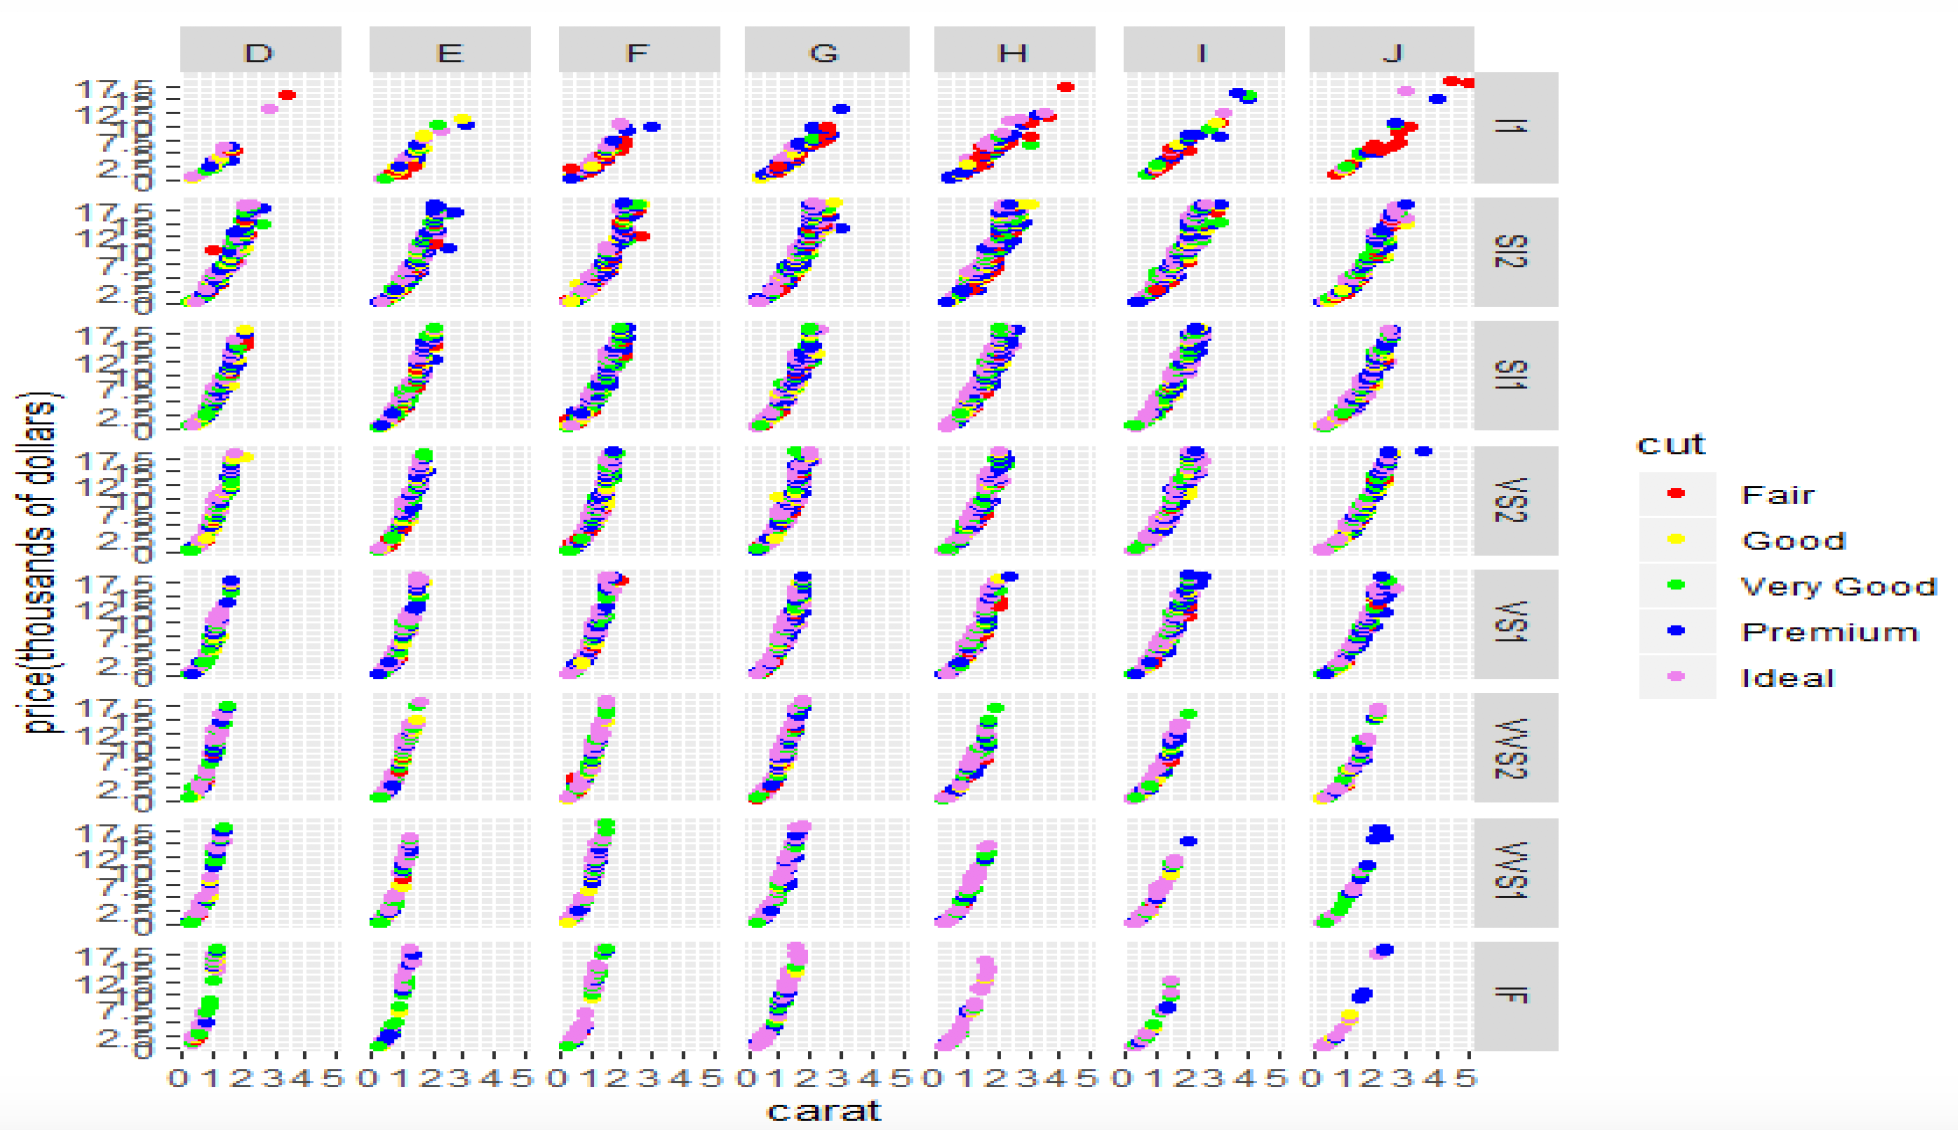
\includegraphics[width=.8\textwidth]{img/sw03/example_02.png}
			\caption{Rendered graph for Second Example}
		\end{figure}
	
		\newpage
		
	\section{Shiny}
	
	Machi de wenni no Loscht han.
	(Wenn de Text am Schloss no do esch, hani kei Loscht meh gha)
	%TODO
	
	\section{Intro to Forecasting}
	
		\subsection{Indication}
		
		\begin{itemize}
			\item Forecast: the ability to use a set of variables for predicting another one
			\item Predictors $\rightarrow$ $F(x)$ $\rightarrow$ Output
			\item Can assume two forms:
				\begin{itemize}
					\item Continuous Output $\rightarrow$ Regression
					\item Discrete (Categorical) Output $\rightarrow$ Classification
				\end{itemize}
			\item It uses similar approaches, but with a different result
			\item The function $F(x)$ is called the model.
				Can be used for two goals:
				\begin{itemize}
					\item Pure prediction: care only for the forecast
					\item Interpretation: care of the existing relationship, to better understand the phenomena
				\end{itemize}
		\end{itemize}
	
		\subsection{Linear Modeling}
		
			\subsubsection{Modeling}
			
			\begin{itemize}
				\item Simplest form of a model is the Linear Model
				\item With one predictor (bidimensional space) represent the equation of a line: \\
					$ y = F(x) = \beta_0 + \beta_1 \cdot x $ \\
			\end{itemize}
		
			\begin{minipage}[c]{0.4\textwidth}
				\centering
				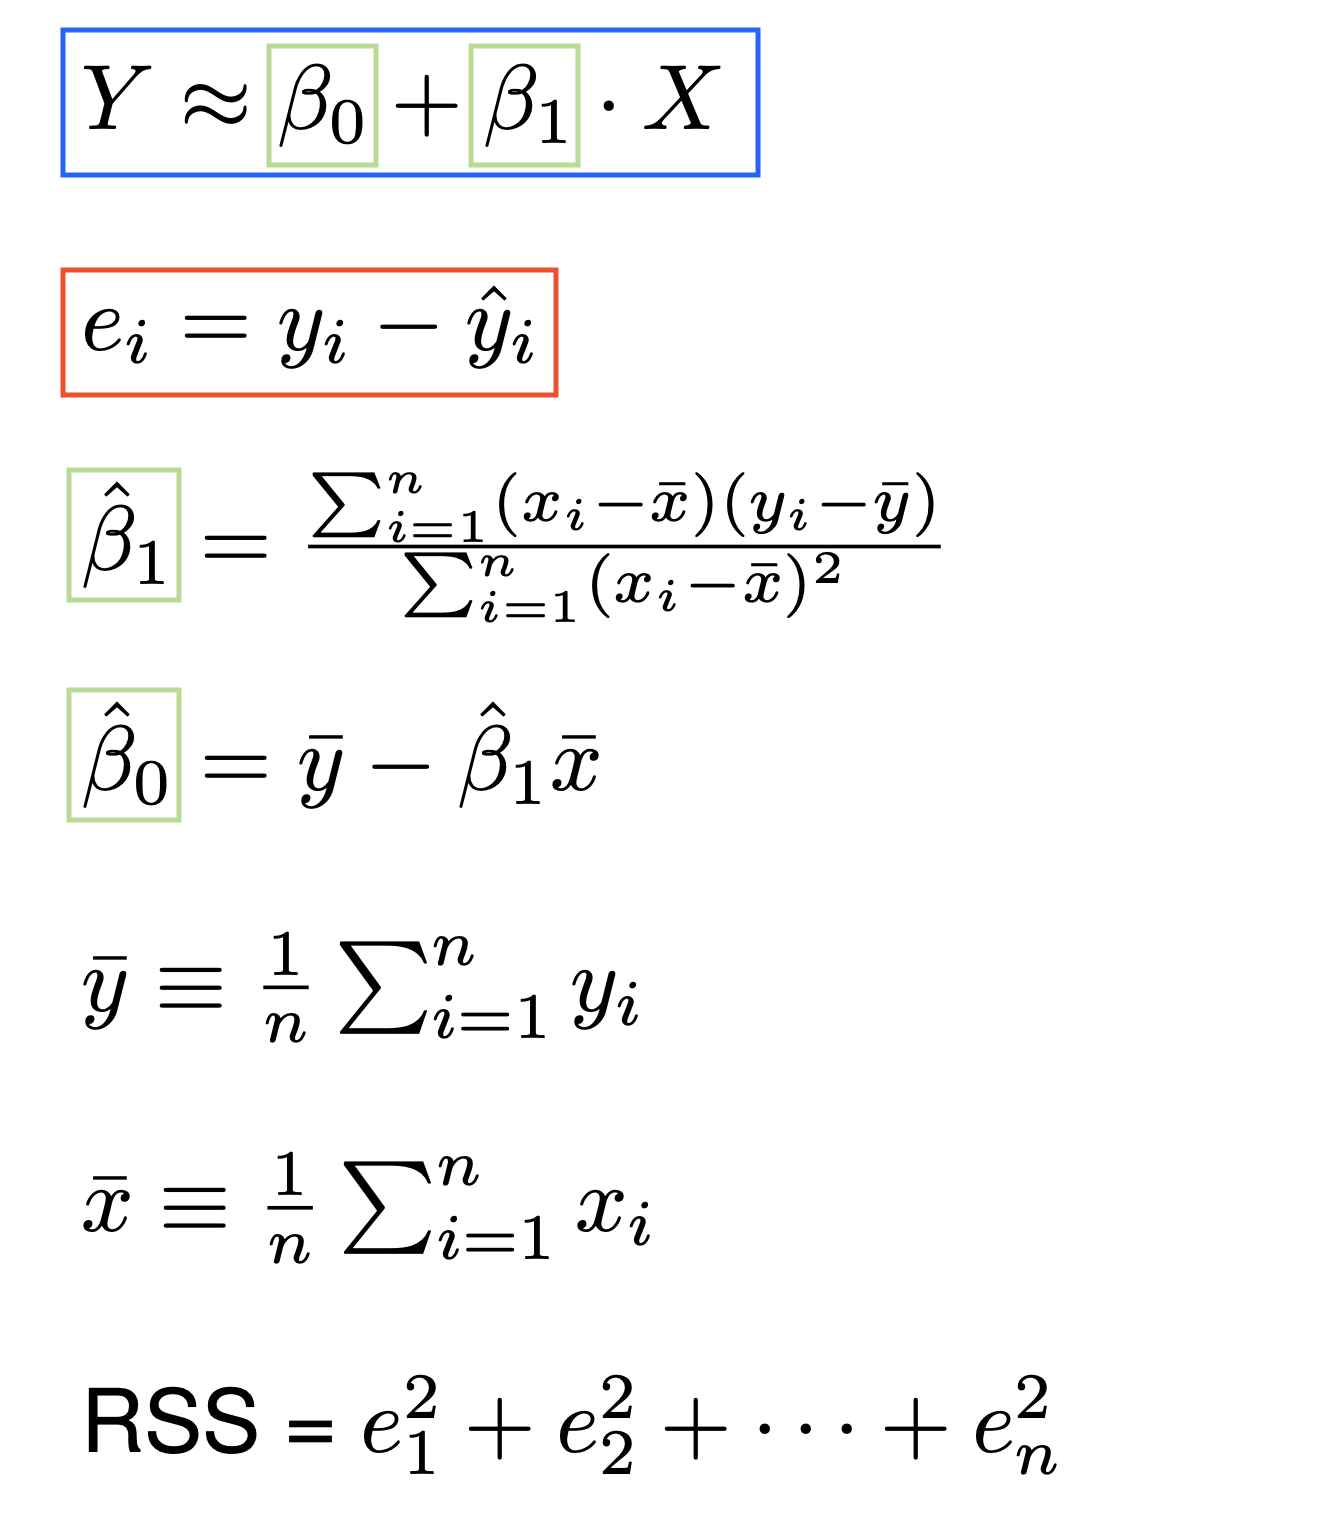
\includegraphics[width=\textwidth]{img/sw08/linear_equations.png}
			\end{minipage}
			\hfill
			\begin{minipage}[c]{0.5\textwidth}
				\centering
				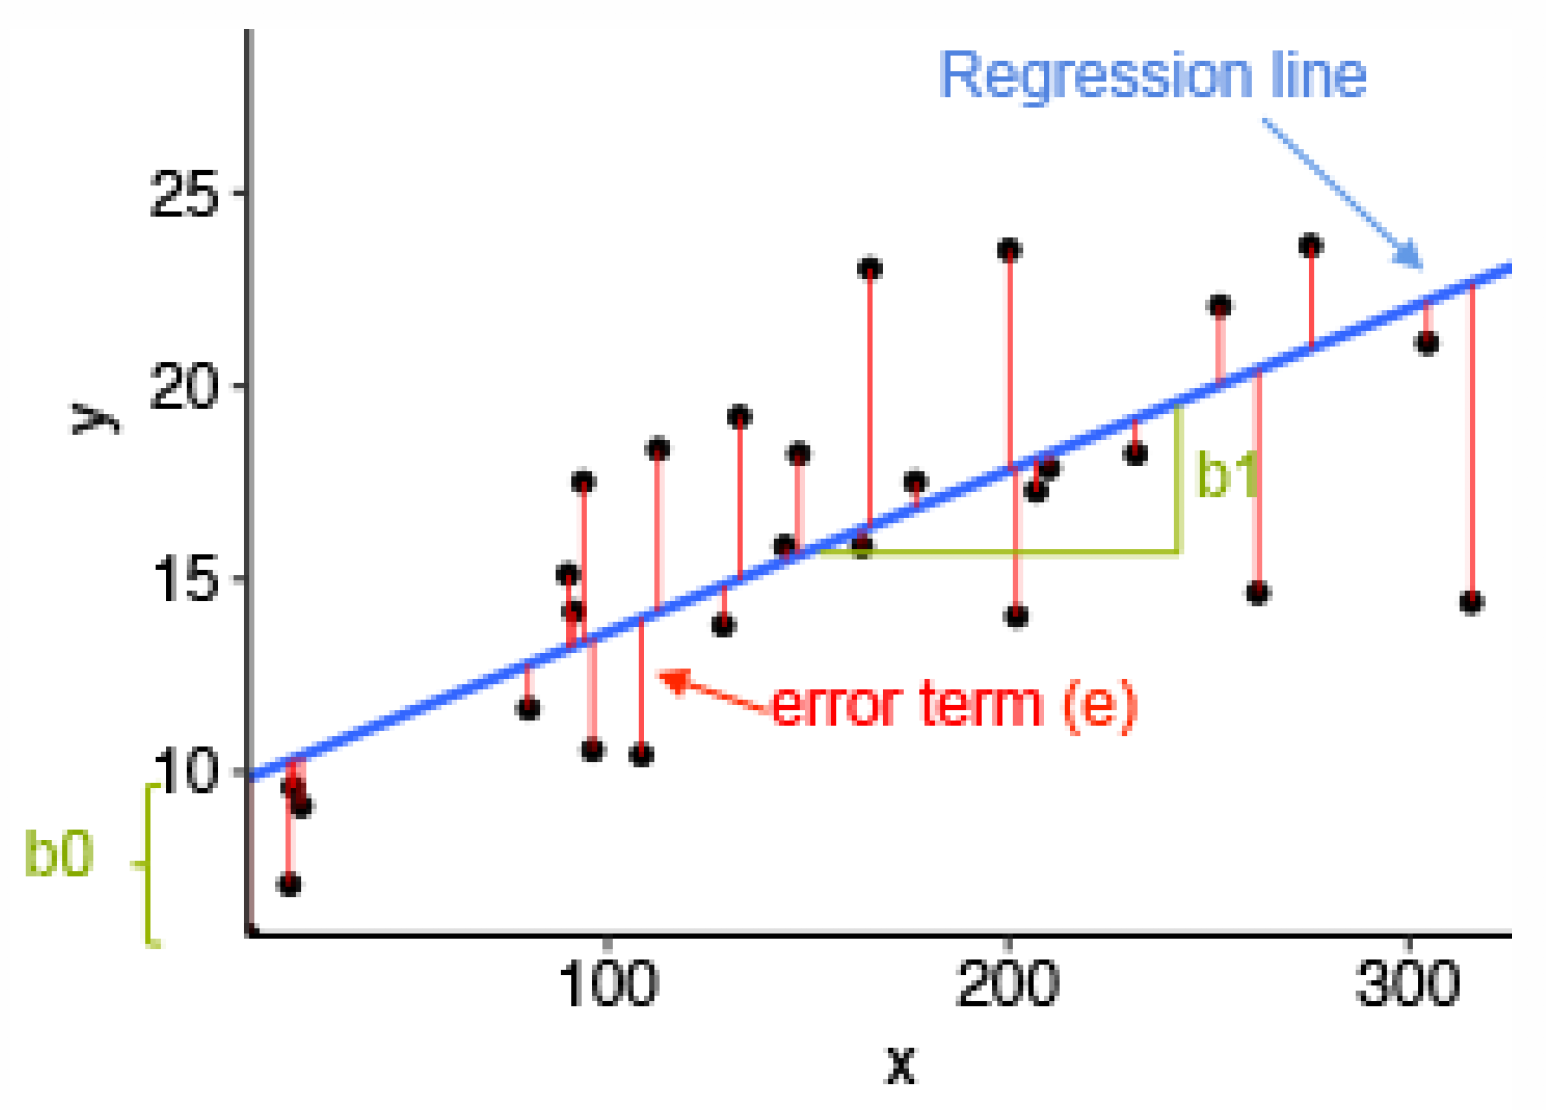
\includegraphics[width=\textwidth]{img/sw08/linear_model.png}
			\end{minipage}
		
			\begin{itemize}
				\item With more predictors (multidimensional space or Hyperspace), \\
					the model can be seen as a hyperplane: \\
					$ y = F(x) = \beta_0 + \beta_1\cdot + \beta_2 \cdot x_2 + \dots + \beta_n \cdot x_n $
			\end{itemize}
		
			\begin{figure}[htb!]
				\centering
				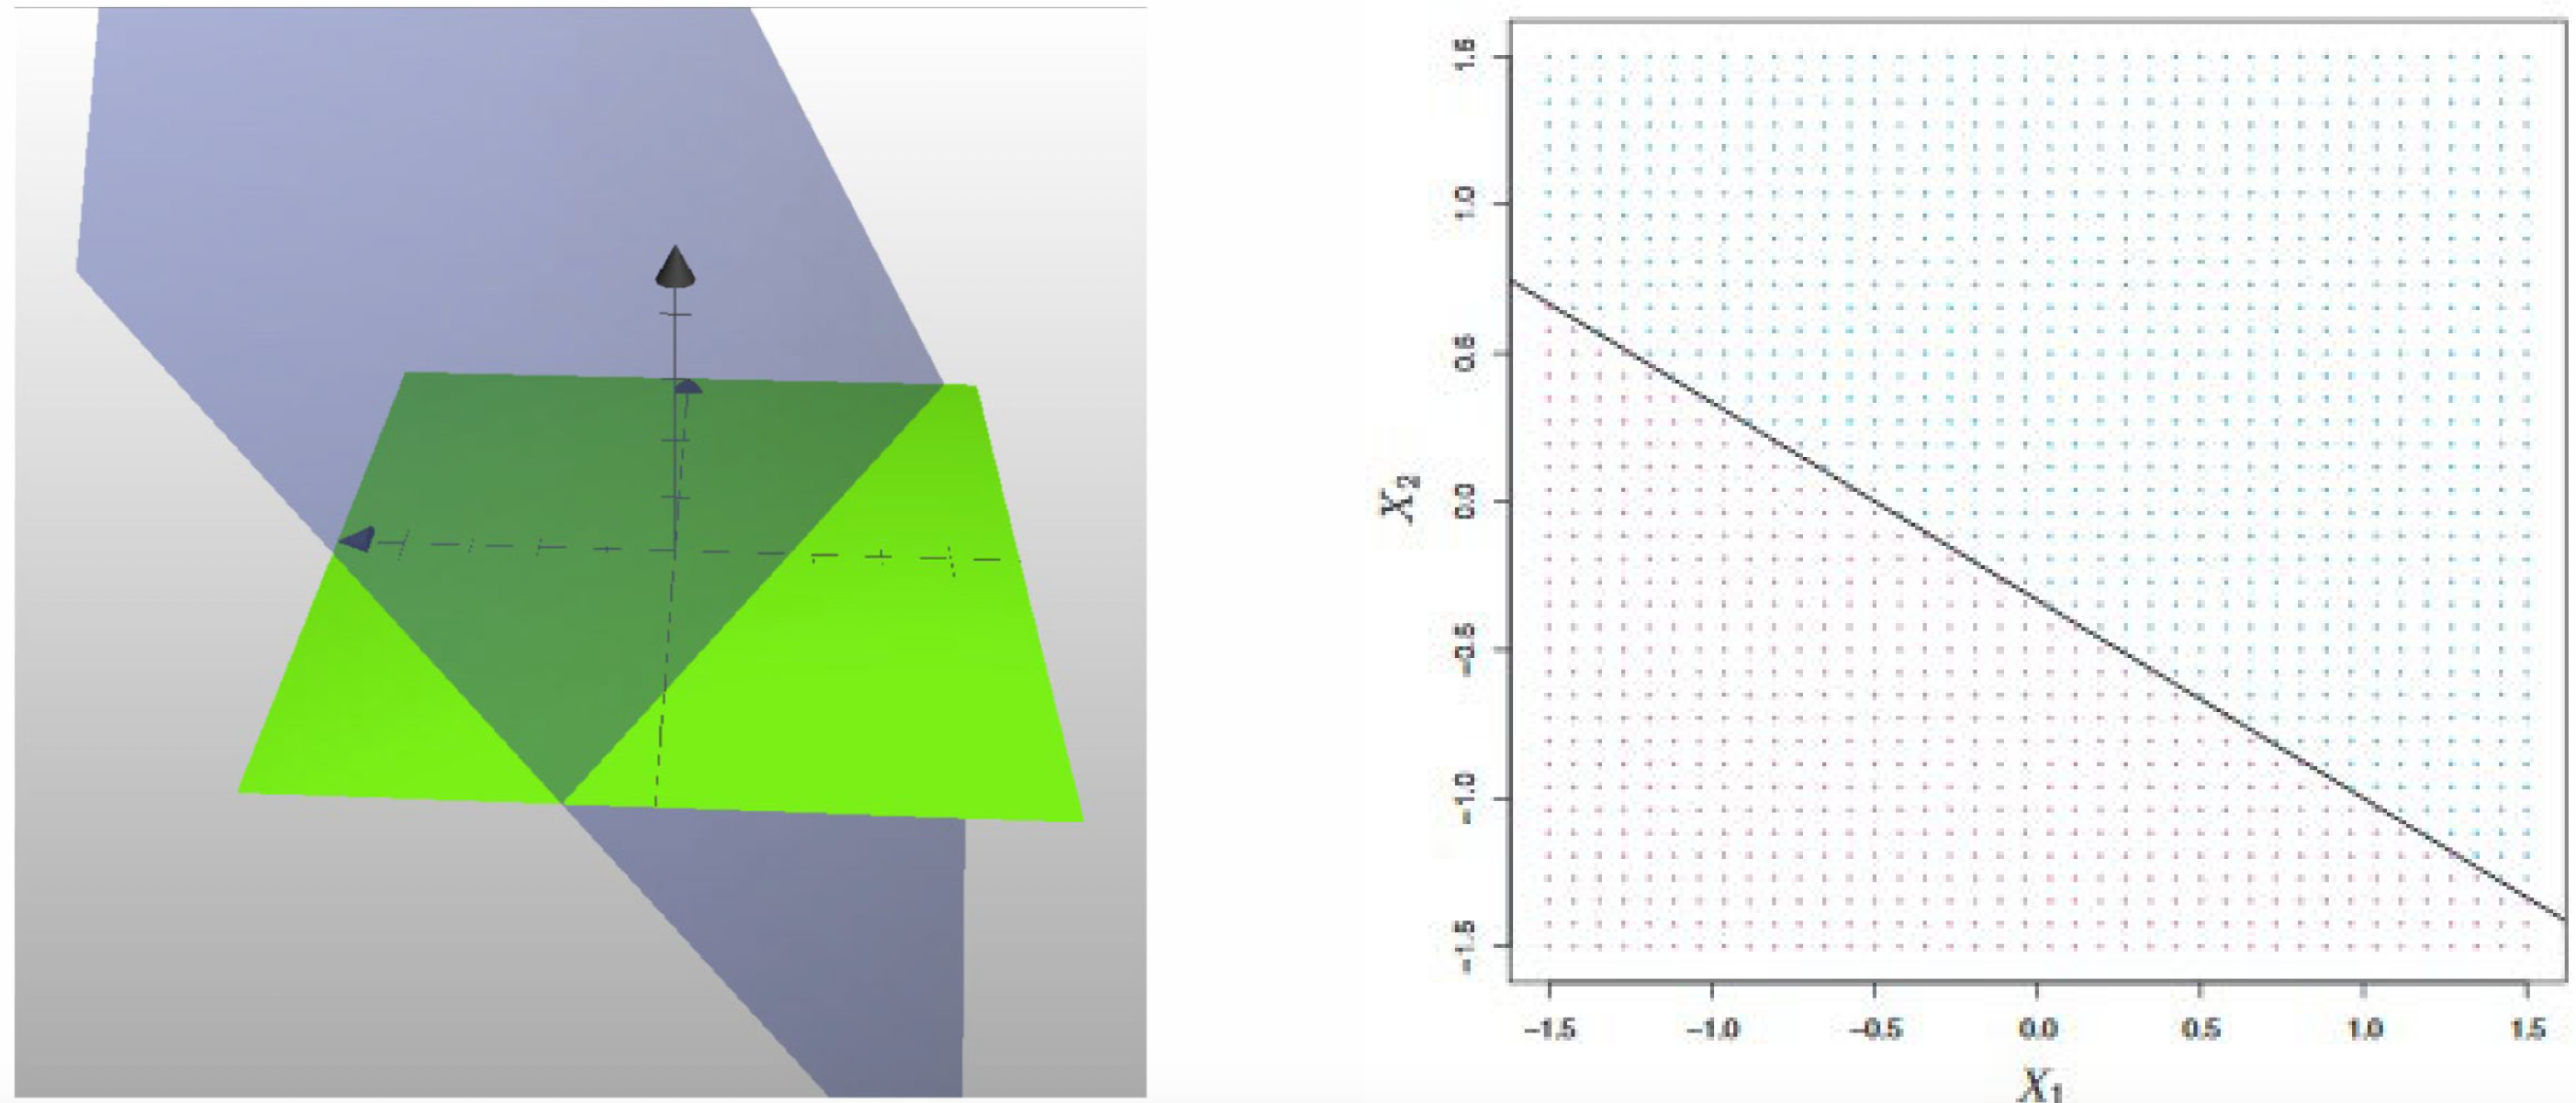
\includegraphics[width=.65\textwidth]{img/sw08/hyperplane.png}
			\end{figure}
		
			\newpage
			
			\subsubsection{Model Identification}
			
			Following steps need to be done
				\begin{itemize}
					\item Define the predictors set and the output variables (also using correlation)
						\begin{itemize}
							\item $x = \dots$, $y = \dots$
						\end{itemize}
					\item Create the model
						\begin{itemize}
							\item \texttt{model <- lm(y \textasciitilde{} x, data = d)}
						\end{itemize}
					\item Inspect the model
						\begin{itemize}
							\item Parameters $\beta_0, \beta_1, \beta_2, \dots, \beta_n$
						\end{itemize}
					\item Verify that the model is "trustable"
						\begin{itemize}
							\item P-values of each $\beta_a$, everyone should be under 0.05 (5\%)
						\end{itemize}
				\end{itemize}
			
			\subsubsection{Prediction}
			
			\begin{itemize}
				\item It is natural to interpret the model for regression:
					\begin{itemize}
						\item Given a single set of predictor values $X$ (point) $\rightarrow$ compute the value of the output ($y$)
					\end{itemize}
				\item but what about for classification?
					\begin{itemize}
						\item We need to define a way to transform the output of the linear model to our output categories
						\item This is done by the logistic function
					\end{itemize}
				\item How to do predictions:
					\begin{itemize}
						\item \texttt{Pred <- predict(model, data = d2)}
					\end{itemize}
			\end{itemize}
				
			\begin{figure}[htb!]
				\centering
				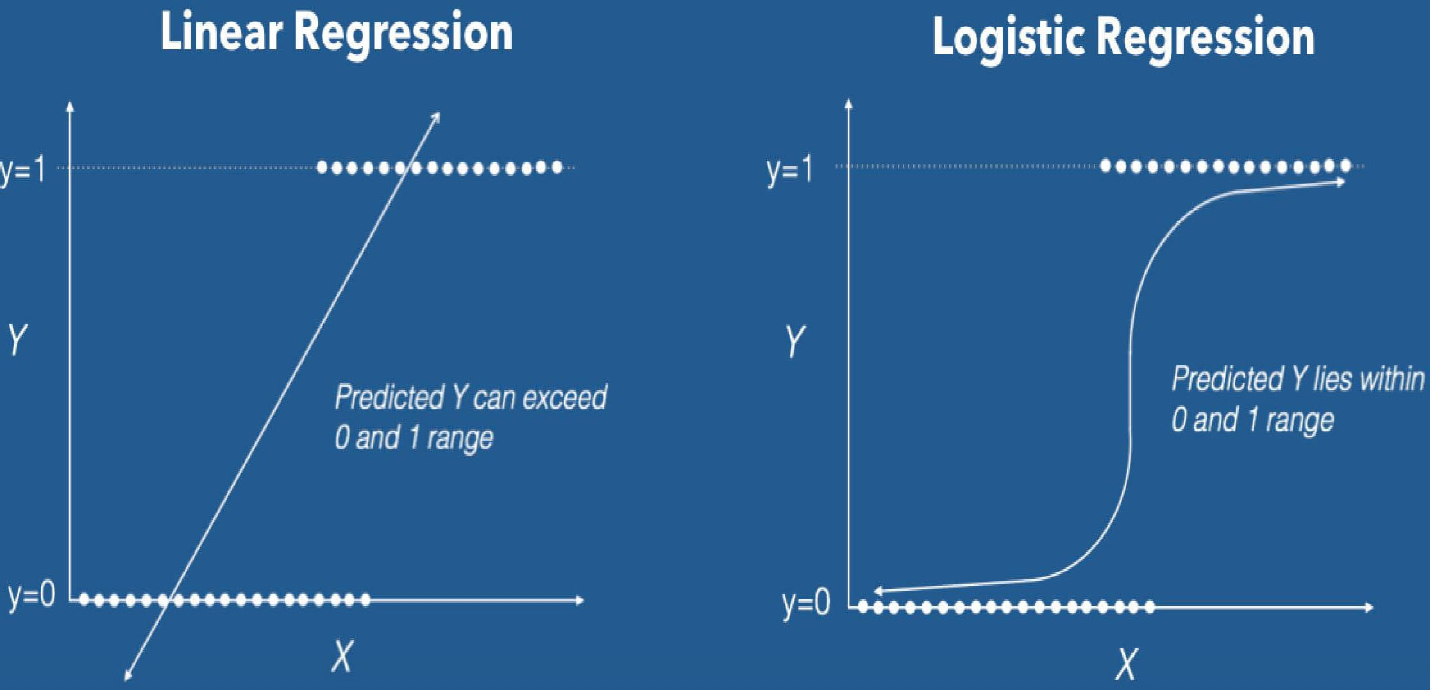
\includegraphics[width=.6\textwidth]{img/sw08/prediction.png}
			\end{figure}
		
			\subsubsection{Model Evaluation}
			
			\begin{itemize}
				\item We need to evaluate models based on performances
					\begin{itemize}
						\item Regression $\rightarrow$ the sum of squared errors (RSS $\rightarrow$ residual sum of squares)
						\item Classification $\rightarrow$ the misclassification error rate
					\end{itemize}
				\item Every model with more predictors has a higher predictive power... \\
					...but, we don't want to learn the noise on the data!
				\item Create an independent test set
					\begin{itemize}
						\item Use most part (e.g. 70\%) of the data for training purposes
						\item Use the rest for the model performance estimation $\rightarrow$ Test Error Rate
					\end{itemize}
			\end{itemize}
		
			\newpage
				
				
				
				
				
				
\end{document}
